\RequirePackage{fix-cm}

% \documentclass{svjour3}                  % onecolumn (standard format)
% \documentclass[smallcondensed]{svjour3}  % onecolumn (ditto)
% \documentclass[smallextended]{svjour3}   % onecolumn (second format)
\documentclass[twocolumn]{svjour3}       % twocolumn
% \documentclass[referee]{svjour3}         % referee (bigger interline spacing)

\smartqed  % flush right qed marks, e.g. at end of proof

\usepackage{graphicx}


% \usepackage{mathptmx}      % use Times fonts if available on your TeX system

% insert here the call for the packages your document requires
\usepackage{fancyvrb}
\usepackage{float}
\usepackage{hyperref}
\usepackage{natbib}

\hypersetup{
  colorlinks=true,
  linkcolor=blue,
  citecolor=blue,
  urlcolor=blue 
}

% please place your own definitions here and don't use \def but
% \newcommand{}{}

% Insert the name of "your journal" with
\journalname{International Journal of Data Science and Analytics}

\begin{document}


\title{A Data Science Approach to Implementing Decision Analytics for Strategic Sourcing\thanks{TBD.}}
% \subtitle{Do you have a subtitle?\\ If so, write it here}

\titlerunning{Decision Analytics for Strategic Sourcing}  % if too long for running head

\author{
  Bradley C. Boehmke \and
  Benjamin T. Hazen \and
  Brandon M. Greenwell \and
  Andrew J. McCarthy
}

%\authorrunning{Short form of author list} % if too long for running head

\institute{Bradley C. Boehmke \at
           Air Force Institute of Technology \\
           2950 Hobson Way \\
           Wright-Patterson AFB, OH 45433 \\
           United States of America \\
           \email{bradleyboehmke@gmail.com} \\
           \and
           Benjamin T. Hazen \at
           Air Force Institute of Technology \\
           2950 Hobson Way \\
           Wright-Patterson AFB, OH 45433 \\
           United States of America \\
           \email{benjamin.hazen@live.com} \\
           \and 
           Brandon M. Greenwell \at
           Illumination Works \\
           6289 Commons Blvd \\
           Suite 120 \\
           Beavercreek, OH 45431 \\
           \email{greenwell.brandon@gmail.com}
           \and
           Andrew McCarthy \\
           The Perduco Group \\
           3610 Pentagon Blvd \\
           Suite 110 \\
           Beavercreek, OH 45431 \\
           \email{andymc82000@yahoo.com}
}

\date{Received: date / Accepted: date}
% The correct dates will be entered by the editor


\maketitle


%%%%%%%%%%%%%%%%%%%%%%%%%%%%%%%%%%%%%%%%%%%%%%%%%%%%%%%%%%%%%%%%%%%%%%%%%%%%%%%%
\begin{abstract}
%%%%%%%%%%%%%%%%%%%%%%%%%%%%%%%%%%%%%%%%%%%%%%%%%%%%%%%%%%%%%%%%%%%%%%%%%%%%%%%%

Data science has emerged as a significant capability upon which firms compete. Although many data scientists and the high-performing companies that employ them seem to have developed robust methods to employ data sciences practices to achieve competitive advantages, there have been few attempts at defining and explaining how and why data science helps firms to achieve desired outcomes.  In this paper, we describe how data science, which combines computer programming, domain knowledge, and analytic skillsets to scientifically extract insights from data, can be used to help meet the growing demand of analytic needs across an organization's value chain. This is done through the illustration of an applied data science initiative to a strategic sourcing problem via the use of open-source technology. In doing so, we contribute to the growing data science literature by demonstrating the application of unique data science capabilities. Moreover, the paper provides a tutorial on how to use a specific R package along with an actual case in which that package use used.

\keywords{Data Science \and Purchasing portfolio \and Supply chain management \and Open source \and R programming \and Decision support}

\end{abstract}


%%%%%%%%%%%%%%%%%%%%%%%%%%%%%%%%%%%%%%%%%%%%%%%%%%%%%%%%%%%%%%%%%%%%%%%%%%%%%%%%
\section{Introduction}
\label{intro}
%%%%%%%%%%%%%%%%%%%%%%%%%%%%%%%%%%%%%%%%%%%%%%%%%%%%%%%%%%%%%%%%%%%%%%%%%%%%%%%%

Organizations increasingly rely upon advanced analytic methods to create insights that lead to competitive advantage \citep{wf13-2,ll13}. Unfortunately, today's organizations often lack the available talent to execute advanced analytics functions \citep{dp12}. Also considering budget constraints, only a few companies possess adequate time and resources to apply analytic approaches to emerging supply chain problems and opportunities \citep{bj16}. In the past, organizations could employ statisticians and operations researchers to explore datasets manually. However, the volume of data and the increasing need for analytics across all supply chain processes has far outstripped the capacity of individual analysts \citep{pf13}. This is not to say that statistician and operations research analysts are under performing.  Rather, in today's data driven environment, organizations are demanding more from their analysts than can be supplied.  In sum, organizations have a need to integrate low-cost, high-level analytics that can be carried out in a timely manner - all while using the minimum amount of expert human capital.
Extant literature emphasizes this need to understand how organizations can better integrate and leverage advanced analytics \citep{ss15}. Researchers are actively building a robust body of knowledge in areas such as:
\begin{enumerate}
  \item Advantages and challenges in the current analytics environment \citep{mb12,ots12,wgnp16},
  \item How data management is changing with today's "big" data environment \citep{cz14,wssa15,rmha16},
  \item How analytic techniques are advancing in conjunction with current technology \citep{hsbh16,wf13,wgnp16},
  \item How education is changing to accommodate the age of big data and data science \citep{ss15,dg15,gk14}.
\end{enumerate}
However, much of this literature lacks practical knowledge and application that can inform today's organizations. \citet{hsbh16} discuss the misalignment between the work of operations research (OR) scholars and the needs of practitioners. Additional literature discusses the lack of exemplar case studies to illustrate how organizations can deploy analytic applications to turn data assets into insights to gain competitive advantages \citep{gh14,p14,wgnp16}.  Without practical applications illustrating the process of orchestrating analytic applications, the gap between research, practice, and impact will only widen \citep{rmha16}.  As Narasimhan warns,
\begin{quote}
How long can a maturing discipline continue to ignore relevance and create 'theories' that are publishable (and indeed published) but don't add to practical knowledge or that are not put to use? We risk becoming irrelevant to industry if we continue down this path of disregard for the usefulness of the knowledge that we create \citep{smbdel15}.
\end{quote}
The purpose of this paper is to address this concern by illustrating how advancements in analytic approaches can become more practical by leveraging open-source technology. In particular, we demonstrate how data science, an interdisciplinary field that combines computer programming, domain knowledge, and analytic skillsets to develop, automate, and deploy scientific methods to extract insights from data, can be used to help meet the growing demand of analytic needs across an organization's value chain. This demonstration of data science capabilities has largely remained absent in the literature, and is therefore the primary contribution of this paper.   Herein, we introduce a novel analytic approach for analyzing an organization's purchasing portfolio in an environment that is efficient, effective, and practical to deploy.  As an exemplar, we illustrate the case of how the open source R programming language is used to package this analytic framework so that analysts can easily and quickly quantify and analyze their organization's purchasing portfolio.  


%%%%%%%%%%%%%%%%%%%%%%%%%%%%%%%%%%%%%%%%%%%%%%%%%%%%%%%%%%%%%%%%%%%%%%%%%%%%%%%%
\section{Data Science and Open Source Software}
\label{sec:2}
%%%%%%%%%%%%%%%%%%%%%%%%%%%%%%%%%%%%%%%%%%%%%%%%%%%%%%%%%%%%%%%%%%%%%%%%%%%%%%%%

Organizations that are able to leverage the deluge of data are proving to be more dynamic and competitive than those that do not \citep{mb12}.  In fact, top performing organizations are embracing data-driven decision-making \citep{mb12} to achieve a decisive competitive advantage over rivals by way of increased productivity, efficiency, profitability and real-time knowledge \citep{tmdl10,mcbbdr}.  


%%%%%%%%%%%%%%%%%%%%%%%%%%%%%%%%%%%%%%%%%%%%%%%%%%%%%%%%%%%%%%%%%%%%%%%%%%%%%%%%
\subsection{Data Science}
\label{sec:2.1}
%%%%%%%%%%%%%%%%%%%%%%%%%%%%%%%%%%%%%%%%%%%%%%%%%%%%%%%%%%%%%%%%%%%%%%%%%%%%%%%%

Data in a vacuum are worthless \citep{gm15}, which necessitates the need to employ the information processing capability known as data science to turn data, both big and small, into decision-making insights. The data science movement continues to grow with the emergence of a variety of new academic programs and industry initiatives \citep{d15,ss15}. Data science has a strong reliance on analytical and computational skills; however, deep domain knowledge is equally important \citep{wf13}.  As echoed by \citet[p. 95]{smbdel15}, "coming up with a good algorithm involves both code and context, a mingling of the complementary strengths of computer scientists and humanists." Figure~\ref{fig:1} illustrates how three primary skillsets converge to make data science.

\begin{figure}[!htb]
  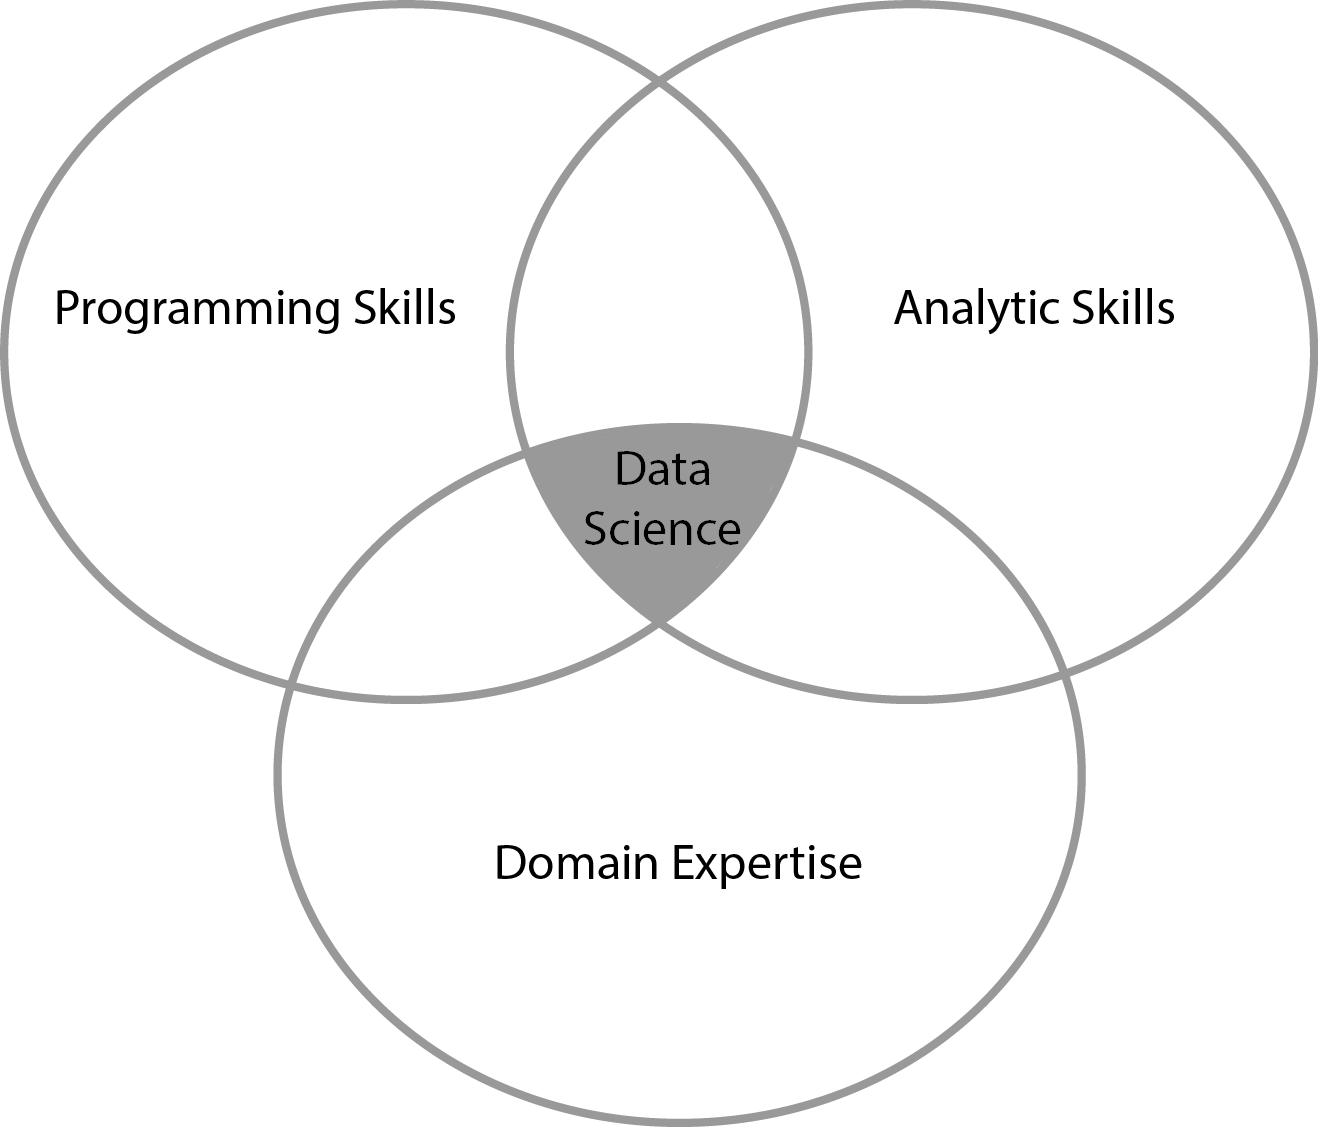
\includegraphics[width=0.5\textwidth]{venn-diagram.png}
  \caption{Components of Data Science.}
  \label{fig:1}
\end{figure}

Although simplified, this illustration points out that to understand the impact of data science, research must illustrate how programming and analytic skills integrate with domain expertise to provide viable solutions to well-defined problems. The application of analytics to domain problems is not new.  In fact, the application of OR dates back to pre-World War II \citep{l84}.  However, what is new is the significant increase that computer programming is playing in modern analytics.  As \citet[p. 74]{dp12} state, the "data scientist's most basic, universal skill is the ability to write code".  This has driven advancements in both the type of analytic techniques applied (i.e., machine learning, natural language processing) and how software is leveraged to produce analytic products, providing organizations greater analytic capabilities. For a complete and thorough overview of data science, see \citet{c17}.


%%%%%%%%%%%%%%%%%%%%%%%%%%%%%%%%%%%%%%%%%%%%%%%%%%%%%%%%%%%%%%%%%%%%%%%%%%%%%%%%
\subsection{Open Source Software}
\label{sec:2.2}
%%%%%%%%%%%%%%%%%%%%%%%%%%%%%%%%%%%%%%%%%%%%%%%%%%%%%%%%%%%%%%%%%%%%%%%%%%%%%%%%

Analytic capabilities within organizations have, historically, been dominated by proprietary software technologies. Unfortunately, these technologies often lack availability, innovation, interoperability, and transparency \citep{d17}.  In recent years, there has been an increasing transition away from proprietary software and towards open source software. Open source software is software that is voluntarily developed and extended by users specific to their organization's needs and made freely available to all \citep{o03}.  For analytic purposes, open source software allows analysts to customize analytic processes and products specific to their organization.  Consequently, open source software has emerged as a major cultural and economic phenomenon \citep{lt02} and illustrates the trend toward developing user innovation around analytic capabilities to increase a firm's performance \citep{h09}. This collaborative model offered by the open source ecosystem can potentially change the analytic nature of organizations by increasing innovation and technology adoption while being constrained by resources \citep{h11}.  

The transition towards open source software also provides an avenue for academia and industry to become better aligned. In addition to advancing analytic methodologies, academics can use open source technology to better operationalize and embed analytic approaches into systems and business processes \citep{ll13}.  Not only does the use of open source software enable faster technology transfer, and easier integration, but resource-constrained organizations of all sizes can also use open source software to develop additional analytic capabilities at lower costs.  Unfortunately, research regarding how open source software can be leveraged by organizations for analytic and decision-making purposes is lacking \citep{bh17}.


%%%%%%%%%%%%%%%%%%%%%%%%%%%%%%%%%%%%%%%%%%%%%%%%%%%%%%%%%%%%%%%%%%%%%%%%%%%%%%%%
\subsection{Open Source for Data Science}
\label{sec:2.3}
%%%%%%%%%%%%%%%%%%%%%%%%%%%%%%%%%%%%%%%%%%%%%%%%%%%%%%%%%%%%%%%%%%%%%%%%%%%%%%%%

During the last decade, free and open source programming languages such as R and Python have become the most widely used tools for analytics and data science \citep{w14}. Their applications run the gamut from data preprocessing, cleaning, internet data extraction, and visualization to a wide range of analytic tasks such as computational statistics, econometrics, optimization, and natural language processing \citep{b16}. Due to their popularity, flexibility, and open source form, R and Python have become essential analytic software throughout industry, being used by organizations such as Google, Facebook, New York Times, Twitter, Etsy, Department of Defense, and even in presidential political campaigns \citep{b16}. 

One of the key factors for the overall success of these analytic programming languages is the packaging system they provide \citep{t17}. Packages are a way to maintain and exchange collections of functions, data sets, interactive applications, and user documentation.  As peer-reviewed journal articles distribute scientific ideas to others, a package distributes mathematical and statistical methods to others.  Packages provide users the ability to extend and modify the analytic functionality for organizations' and communities' needs while still enforcing programming and quality standards \citep{bj16}.  This provides a convenient way to develop and maintain analytic functions to be shared with colleagues, organizations and other analysis and supply chain community members.  Moreover, this offers an opportunity to transfer analytic functionalities developed by the research community to the practitioners as quickly as (and in some cases even quicker than) ideas and methodologies are transferred via peer-reviewed articles. Furthermore, it has been the authors' experience that most defense organizations, such as the Air Force, Navy, Army, Missile Defense Agency, and the reserve components, primarily rely on Excel for decision analysis modeling.  Unfortunately, Excel provides a very limited environment for developing and sharing analytic functionality. Consequently, each analyst is often left to their own devices to create and implement analytic techniques. This creates several limitations such as consistency and validity of implemented functions and can greatly impede the implementation of newly established analytic techniques.  In some cases proprietary software is relied on; however, proprietary software restricts access to the underlying functions, eliminating the ability to customize the software's capabilities to an organization's needs \citep{bj16}.  Consequently, many organizations pay excessive licensing fees for analytic software that does not provide the outputs desired. It is only realistic that these same challenges exist in most firms performing analytic activities as well.

Open source programming languages and their packaging ecosystem provide the operations research community a free alternative to develop, customize and extend analytic functionality for our organizations and communities with consistent, valid, and swift implementation. And due to its free and open source nature it is readily available for use by organizations across industries. Thus, this collective action capability is primed for implementation within and across the operations research community.  To illustrate, we will demonstrate a data science approach to address a strategic sourcing problem.


%%%%%%%%%%%%%%%%%%%%%%%%%%%%%%%%%%%%%%%%%%%%%%%%%%%%%%%%%%%%%%%%%%%%%%%%%%%%%%%%
\section{Domain Problem: Purchasing Portfolios for Strategic Sourcing}
\label{sec:3}
%%%%%%%%%%%%%%%%%%%%%%%%%%%%%%%%%%%%%%%%%%%%%%%%%%%%%%%%%%%%%%%%%%%%%%%%%%%%%%%%

Business leaders are increasingly reliant upon new forms of data and analytics to gain greater visibility into key activities such as purchasing, operations, logistics, and, product and service development \citep{cps15,hbej14}. Herein, we consider purchasing and strategic sourcing as an application domain. 

Purchasing portfolio models provide an approach for differentiating suppliers \citep{pwa12,md05,br01} and commodities \citep{oe97,ns00}.  Purchasing portfolio models have received considerable attention from academia and within organizations \citep{gv03}.  This attention is driven by the recognition that the ability of the firm to manage supplier relations has been empirically linked to obtaining and sustaining competitive advantage \citep{cpl04,dcc98}. Moreover, suppliers play an increasingly significant role in the success of firms \citep{wj04}. However, all suppliers cannot be dealt with in the same way and the literature supports the need to differentiate supplier relationships through differentiation schemes offered by purchasing portfolio models \citep{gm08,ly01}.  

\citet{k83} introduced the first comprehensive portfolio approach for purchasing and supply management \citep{gv03}.  Although other models have been developed \citep{tj96,dp02,k07}, the Kraljic Portfolio Matrix KPM approach has become the dominant methodology in both literature and practice \citep{lchp01,gv03}. Kraljic's approach leverages a portfolio matrix that classifies products on the basis of two dimensions: the external dimension ('Supply Risk') concerns the factors regarding suppliers and supply market, while the internal dimension ('Profit Impact') relates to the importance and profit impact of a given product \citep{dp02}. Each dimension needs to be assessed against a number of variables where an overall classification score ('low' and 'high') is established. The result is a $2 \times 2$ matrix and a classification in four categories: non-critical, leverage, bottleneck, and strategic items as illustrated in Figure~\ref{fig:2}. This categorization allows commodities to be classified in a way that minimizes the supply risk while maximizing purchasing power and profits of the firm \citep{pwa12}.

\begin{figure}[!htb]
  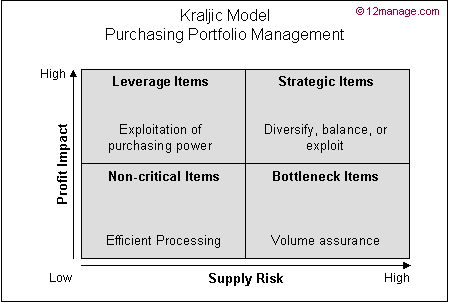
\includegraphics[width=0.5\textwidth]{kraljic-matrix.png}
  \caption{Kraljic Matrix.}
  \label{fig:2}
\end{figure}

There are several variants to the KPM; however, most alternatives build on and extend the KPM by focusing on the factors and variables to be measured.  However, one of the KPM's main critiques revolves around the question: How does a purchasing manager position a product or service within the matrix? \citet{pwa12}, state that "positioning commodities in the KPM suggested in the literature are mainly based on subjective judgment of the decision makers to position the commodities in the different quadrants...They lack analytical rigor, where subjective positioning of commodities may lead to erroneous outcomes." \citet{wj04} add that "Despite the abundance of research on relationship patterns and their impact on company performance, the 'how-to' question has been widely neglected." \citet{r94} identifies an "absence of a conceptual framework to facilitate an analytical approach." \citet{pwa12} add that "positioning of the items in the portfolio matrix by the purchasing managers are subjective and makes the portfolio models imprecise." \citet{ktp14} reiterate the lack of analytical rigor, the difficulty in measuring the matrix dimensions, and the argument "for less subjective methods for positioning purchases on the matrix." \citet{ld10} argue that lack of "the synthesizing of qualitative and quantitative measures" promote arbitrary classification of purchases. \citet{oe97} emphasize that categorizing of "purchases in a portfolio model...is very subjective, and perhaps the most important part" of the implementation process and urge the use of quantitative methodologies.

Although not exhaustive, a review of literature identified only five attempts to use quantitative techniques to position items with the KPM. Three of the five techniques \citep{oe97,lx08,pwa12} rely on the concept of importance weights or importance scoring; \citet{zdl07} apply factor analysis techniques to the dimensions of the KPM. However, the model lacks sufficient detail in derivation of variable scoring and positioning of items, and \citet{ld10} apply the Analytical Hierarchy Process (AHP) to position items. Each of these approaches are not without their flaws (see \citet{dpbhc08, pbtj13, wb87} for limitations in these approaches). However, of greater concern is the ability to extend and deploy these modeling approaches for practical use is limited and its ease of implementation is inadequate. 

Thus, we introduce a multi-objective approach to position and analyze an organization's purchasing portfolio and use the R open source programming language to package and deploy the technique to ease implementation.


%%%%%%%%%%%%%%%%%%%%%%%%%%%%%%%%%%%%%%%%%%%%%%%%%%%%%%%%%%%%%%%%%%%%%%%%%%%%%%%%
\section{The KraljicMatrix Package: A Data Science Solution}
\label{sec:4}
%%%%%%%%%%%%%%%%%%%%%%%%%%%%%%%%%%%%%%%%%%%%%%%%%%%%%%%%%%%%%%%%%%%%%%%%%%%%%%%%

KraljicMatrix \citep{bmof17} is an R package developed by the authors to provide a quantitative framework to position and analyze a firm's purchasing portfolio. Furthermore, it allows an analyst to quickly implement this analysis in a consistent manner. The KraljicMatrix package is available to download from the Comprehensive R Archive Network (CRAN; \url{https://cran.r-project.org} or from the GitHub repository (\url{https://github.com/afit-r/KraljicMatrix}). To install the stable version, which is hosted on CRAN, run:
% \begin{Verbatim}[fontsize=\footnotesize]
% install.packages("KraljicMatrix")
% \end{Verbatim}
\begin{figure}[!htb]
  
\includegraphics[width=0.5\textwidth]{code1.png}
\end{figure}
within the R operating environment. To download the development version, which is hosted on GitHub, run:
% \begin{Verbatim}[fontsize=\footnotesize]
% library(devtools)
% install_github("AFIT-R/KraljicMatrix")
% \end{Verbatim}
\begin{figure}[!htb]
  
\includegraphics[width=0.5\textwidth]{code2.png}
\end{figure}
Now that the package is downloaded, we load the KraljicMatrix package in our current R environment to allow access to the functions:
% \begin{Verbatim}[fontsize=\footnotesize]
% library(KraljicMatrix)
% \end{Verbatim}
\begin{figure}[!htb]
  
\includegraphics[width=0.5\textwidth]{code3.png}
\end{figure}
The KraljicMatrix package has eight functions to aid analysts in performing a KPM analysis:
\begin{table*}[!htb]
  \centering
  \caption{Analytic functions provided by the KraljicMatrix package.}
  \label{tab:1}       % Give a unique label
  \begin{tabular}{lp{10cm}}
    \hline\noalign{\smallskip}
    Function & Purpose  \\
    \noalign{\smallskip}\hline\noalign{\smallskip}
    SAVF\_score & Computes a utility score based on an exponential single attribute value function. \\
    SAVF\_preferred\_rho & Computes the preferred rho that minimizes the squared error between subject matter inputs and exponentially fitted utility scores. \\
    SAVF\_plot\_rho\_error & Plots the squared error terms for the rho search space to illustrate the preferred rho that minimizes the squared error between subject matter desired values and exponentially fitted scores. \\
    SAVF\_plot & Plots the single attribute utility curve along with the subject matter desired values for comparison. \\
    MAVF\_score & Computes the muti-attribute value score based on $x$ and $y$ attribute utility scores and their respective weights. \\
    MAVF\_sensitivity & Computes summary statistics for multi-attribute value scores for $x$ and $y$ given a range of swing weights for each attribute. \\
    kraljic\_quadrant & Identifies the Kraljic purchasing matrix quadrant for each product or service based on the attribute utility scores of $x$ and y. \\
    kraljic\_matrix & Plots each product or service in the Kraljic purchasing matrix based on the attribute value score of $x$ and y. \\
    \noalign{\smallskip}\hline
  \end{tabular}
\end{table*}

Furthermore, an example dataset psc is provided in the KraljicMatrix package. This data contains 200 product and service contracts (PSCs). Each PSC has an $x$ attribute (i.e., supply risk) score from 1 (worst) to 5 (best) and $y$ attribute (i.e., profit impact) score from 1 (worst) to 10 (best).  We will use this data to illustrate the functionality of the KraljicMatrix package.

% \begin{Verbatim}[fontsize=\footnotesize]
% psc
% ## # A tibble: 200 x 3
% ##      PSC x_attribute y_attribute
% ##    <chr>       <int>       <int>
% ## 1   D233        3.01        4.84
% ## 2   F352        4.34        5.64
% ## 3   T713        3.37        4.30
% ## 4   K833        2.67        5.53
% ## 5   Q121        3.48        4.33
% ## 6   C791        3.32        7.32
% ## 7   Y207        3.48        5.42
% ## 8   W439        2.47        3.35
% ## 9   N290        1.66        4.02
% ## 10  C251        1.00        7.47
% ## # ... with 190 more rows
% \end{Verbatim}
\begin{figure}[!htb]
  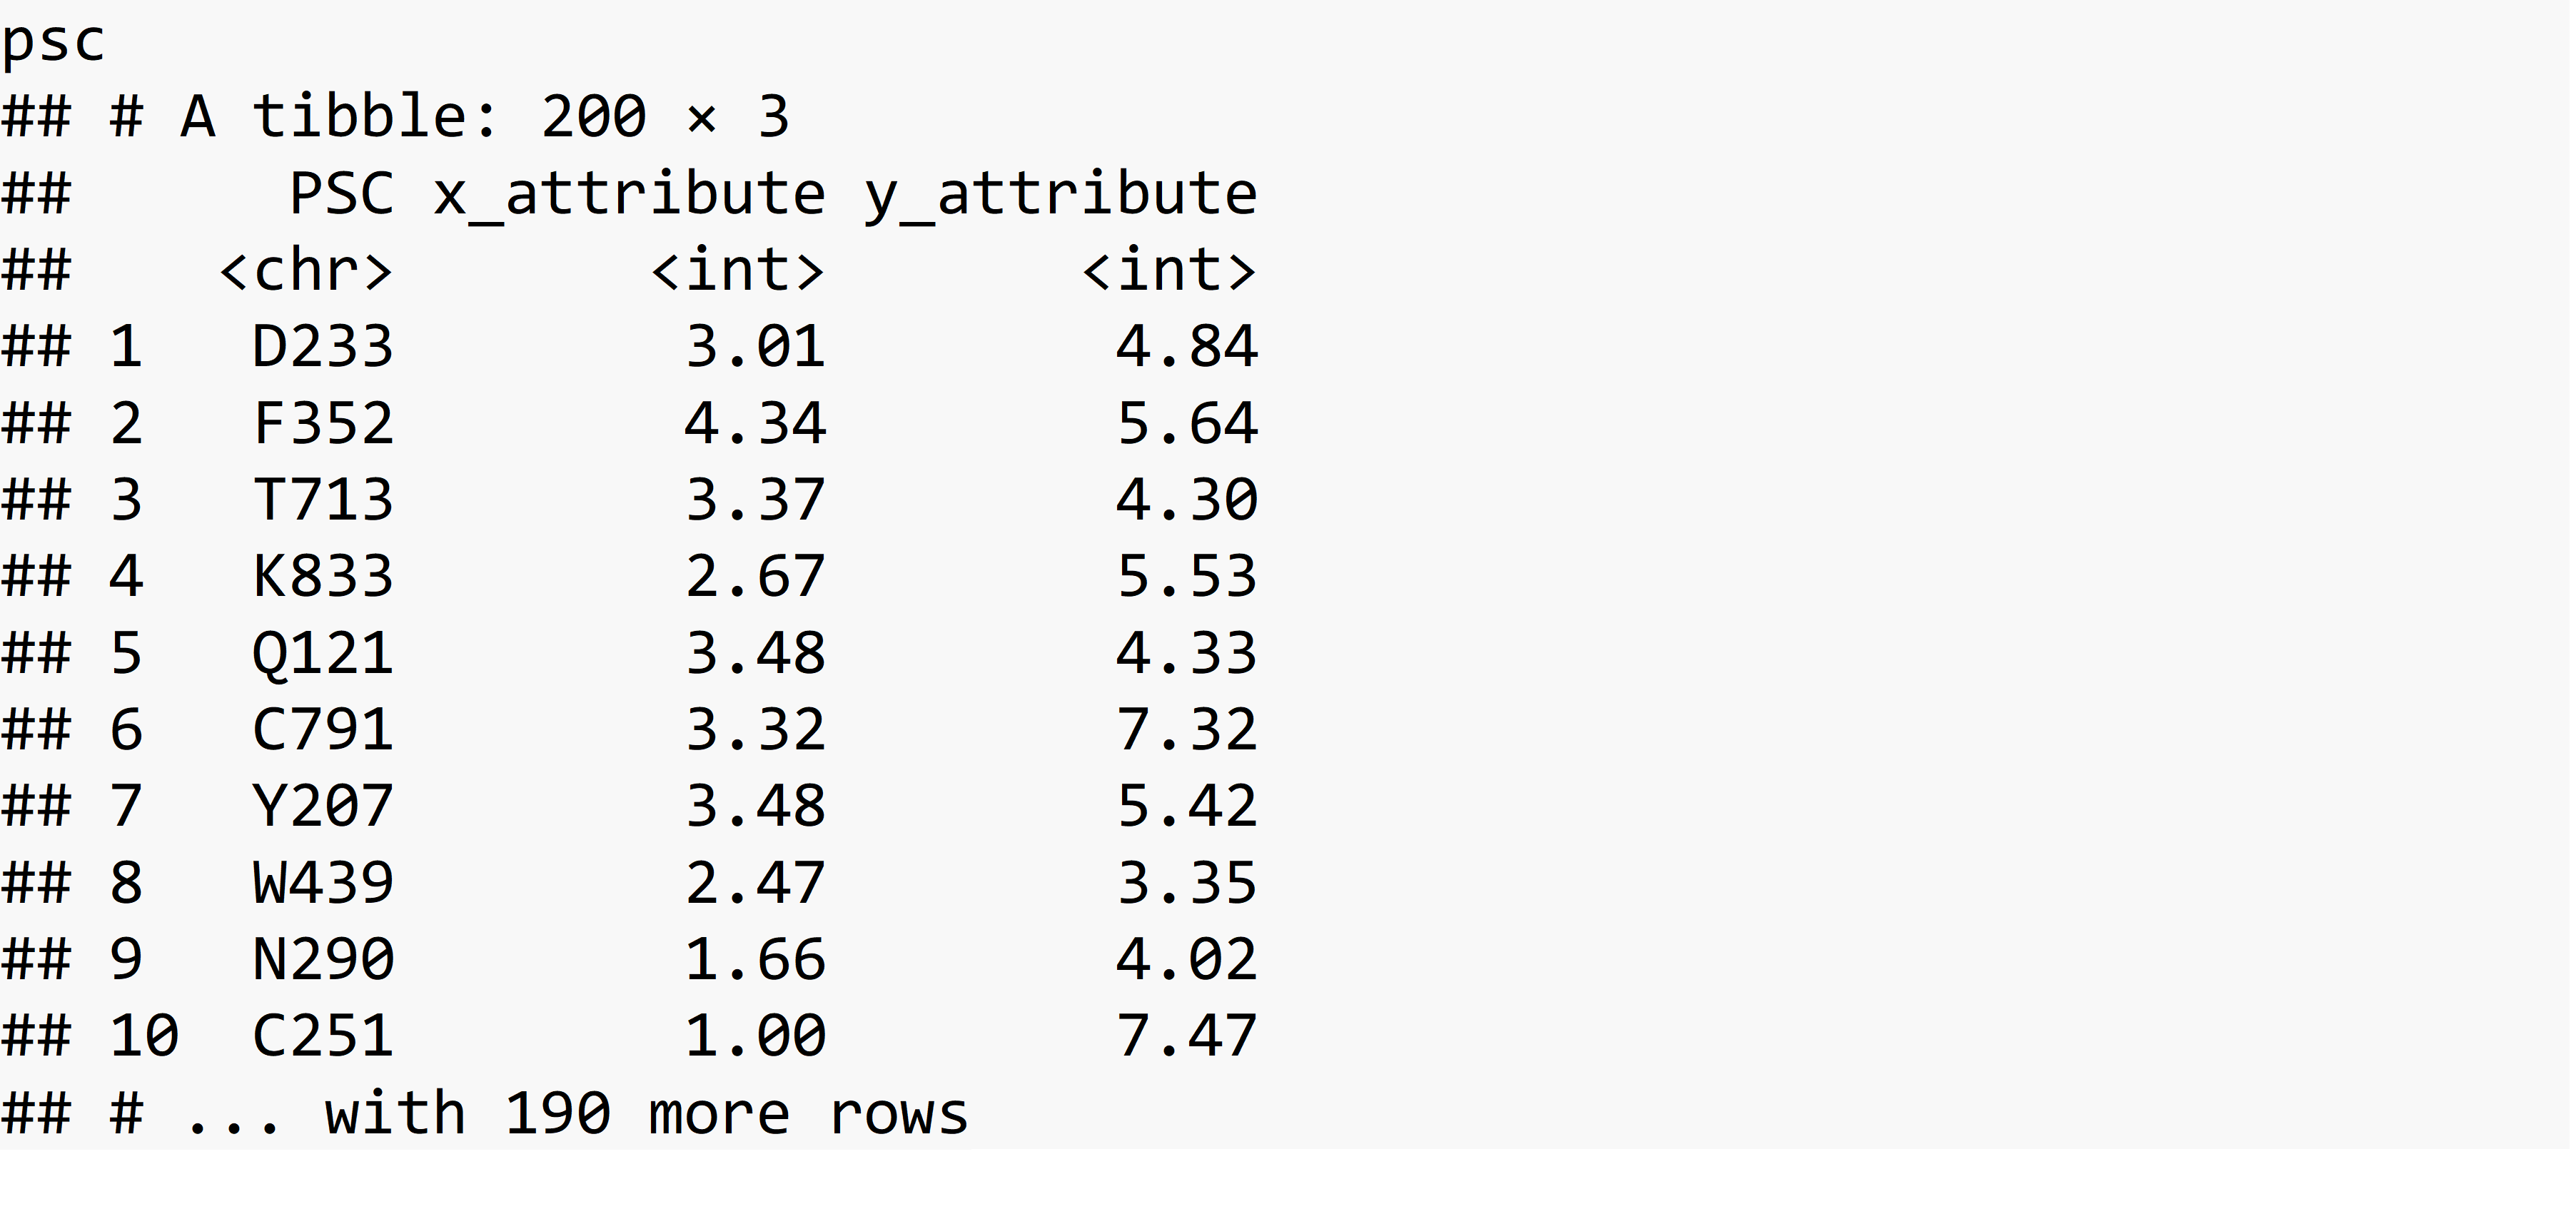
\includegraphics[width=0.5\textwidth]{code4.png}
\end{figure}

First, we must remember that the KPM merely plots products and services on an $x$-$y$ axis coordinate system.  The $x$ and $y$ attributes are simply evaluation measures. They enable each product and service to obtain a score for each dimension being measured. For example, the $x$ attribute score could be the IBISWorld Buyer Power Score measuring supply market complexity (1-5 in 0.01 increments). However, to plot these attributes on the KPM matrix we need to normalize the values scores such that i) the values represent the decision makers' preferences and ii) the values are standardized. To do this we can use an exponential single attribute value function (SAVF). For example, let $0 \le v_x\left(x\right) \le 1$ represent the normalized value of the $x$ attribute such that $x^0$ and $x^*$ are the lowest and highest preferred value of attribute $x$ respectively. Thus, $v_x\left(x^0\right) = 0$ and $v_x\left(x^*\right) = 1$. Consequently, let $v_x\left(x_i\right)$ be the SAVF of exponential form whereby each $x_i$ is an input and $\rho_x$ be the exponential constant for $v_x\left(x_i\right)$:
\begin{equation}
\label{eqn:1}
v_x\left(x_i\right) = \frac{1 - \exp\left(-\left(x_i - x^0\right)\right) / \rho_x}{1 - \exp\left(-\left(x^* - x^0\right)\right) / \rho_x}, \quad \forall i \in A.
\end{equation}

After solving the single attribute value function for both $x$ and $y$ attributes, we obtain a $\left[v_x\left(x_i\right), v_y\left(y_i\right)\right]$ ordered pair for each service or product to be plotted in the KPM.  However, prior to applying the SAVF to our $x$ and $y$ attributes we must first identify the appropriate $\rho$ value. The benefit of applying an exponential SAVF is that it can take on many forms of increasing rates, along with aligning to a linear value function. Consequently, if certain $x$ attribute values are valued more than other values an exponential SAVF will capture this utility curve. To identify the appropriate exponential rate, subject matter expert (SME) inputs are typically evaluated and an exponential rate that most closely matches the preferred values provided by the SMEs is chosen. Thus, let's assume for our given $x$ attribute the SME inputs suggest that $x$ attribute values of 3, 4, and 5 provide a utility score of 0.80, 0.90, and 1.0 respectively (this represents a decreasing rate of return utility curve). Knowing that our $x$ attribute is bounded between 1 and 5 we can search for a $\rho$ value between 0 and 1 that provides the best-fit utility function using the SAVF\_preferred\_rho function.  Best-fit is measured by minimizing the sum of squared residuals ($S = \sum_{i = 1}^n r_i ^ 2$).
% \begin{Verbatim}[fontsize=\footnotesize]
% SAVF_preferred_rho(desired_x = c(3, 4, 5),
%                    desired_v = c(0.8, 0.9, 1),
%                    x_low = 1,
%                    x_high = 5,
%                    rho_low = 0,
%                    rho_high = 1)
% ## [1] 0.6531
% \end{Verbatim}
\begin{figure}[!htb]
  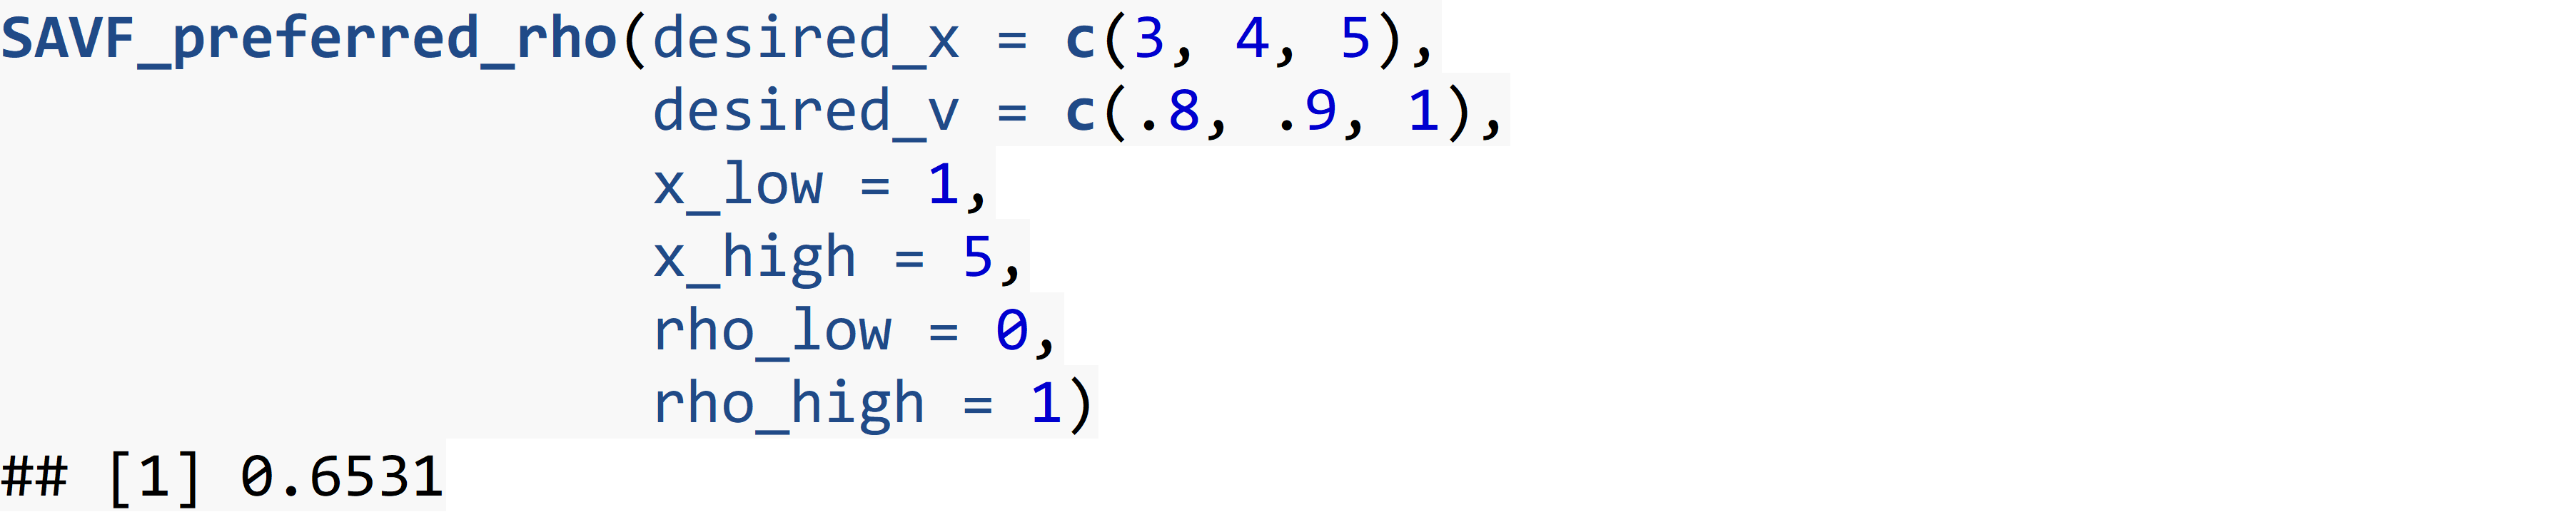
\includegraphics[width=0.5\textwidth]{code5.png}
\end{figure}

Thus, we can see that $\rho = 0.6531$ provides the best-fit exponential SAVF. We can illustrate this two ways. First, we can use SAVF\_plot to plot the single attribute utility curve compared to the subject matter desired values.
% \begin{Verbatim}[fontsize=\footnotesize]
% SAVF_plot(desired_x = c(3, 4, 5),
%           desired_v = c(0.8, 0.9, 1),
%           x_low = 1,
%           x_high = 5,
%           rho = 0.6531)
% \end{Verbatim}
\begin{figure}[!htb]
  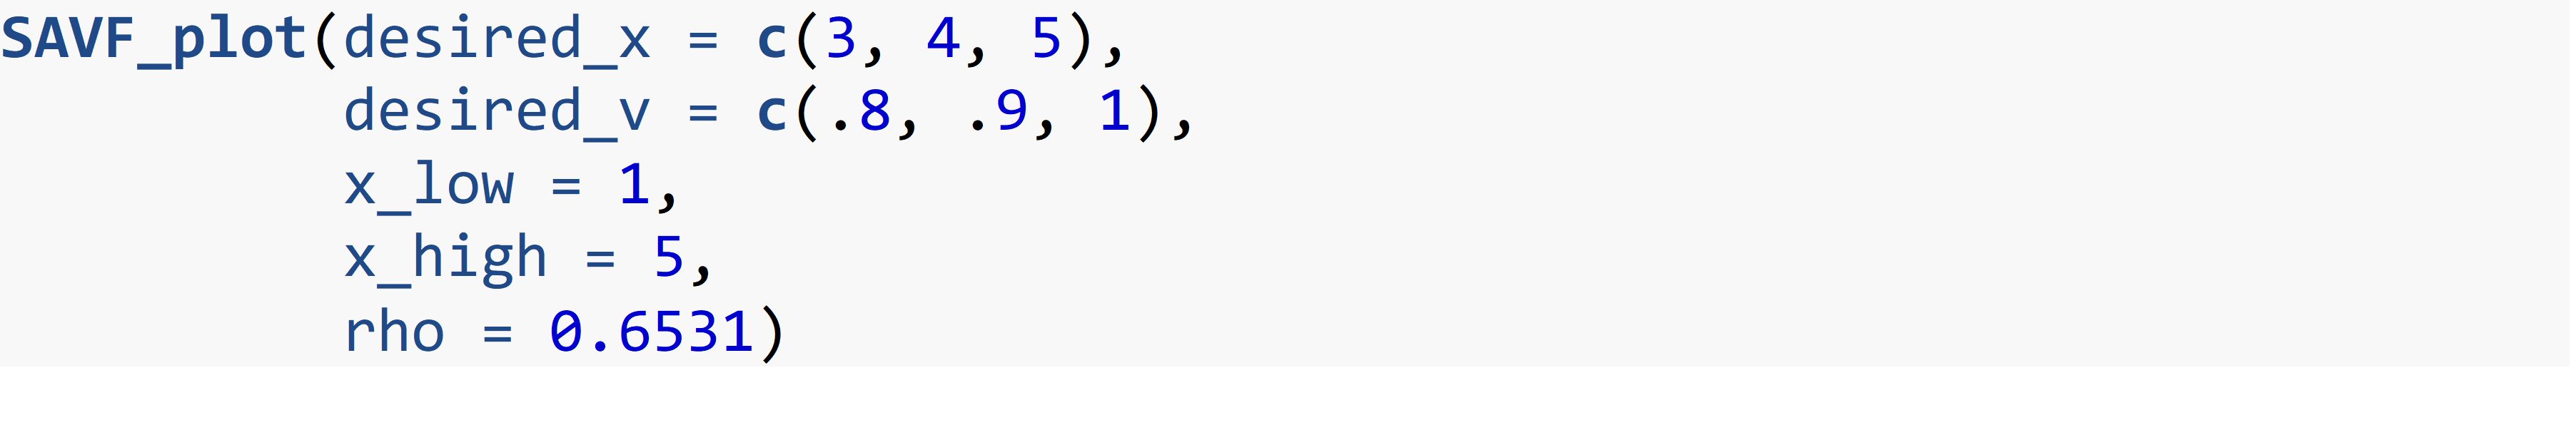
\includegraphics[width=0.5\textwidth]{code6.png}
\end{figure}

\begin{figure}[!htb]
  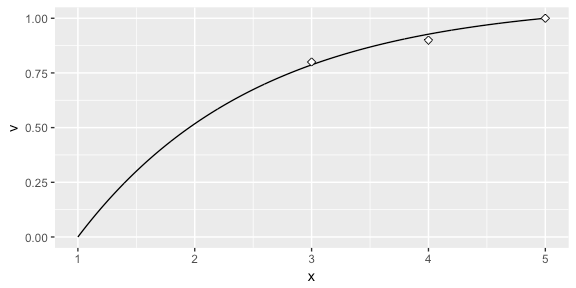
\includegraphics[width=0.5\textwidth]{fig3.png}
  \caption{Single attribute utility curve.}
  \label{fig:3}
\end{figure}

We can also visualize the errors of the $\rho$ search space with SAVF\_plot\_rho\_error, which plots the squared error terms for all $\rho$ values within the $\rho$ search space to illustrate the preferred $\rho$ that minimizes the squared error between subject matter desired values and exponentially fitted scores.
% \begin{Verbatim}[fontsize=\footnotesize]
% SAVF_plot_rho_error(desired_x = c(3, 4, 5),
%                     desired_v = c(.75, 0.9, 1),
%                     x_low = 1,
%                     x_high = 5,
%                     rho_low = 0,
%                     rho_high = 1)
% \end{Verbatim}
\begin{figure}[!htb]
  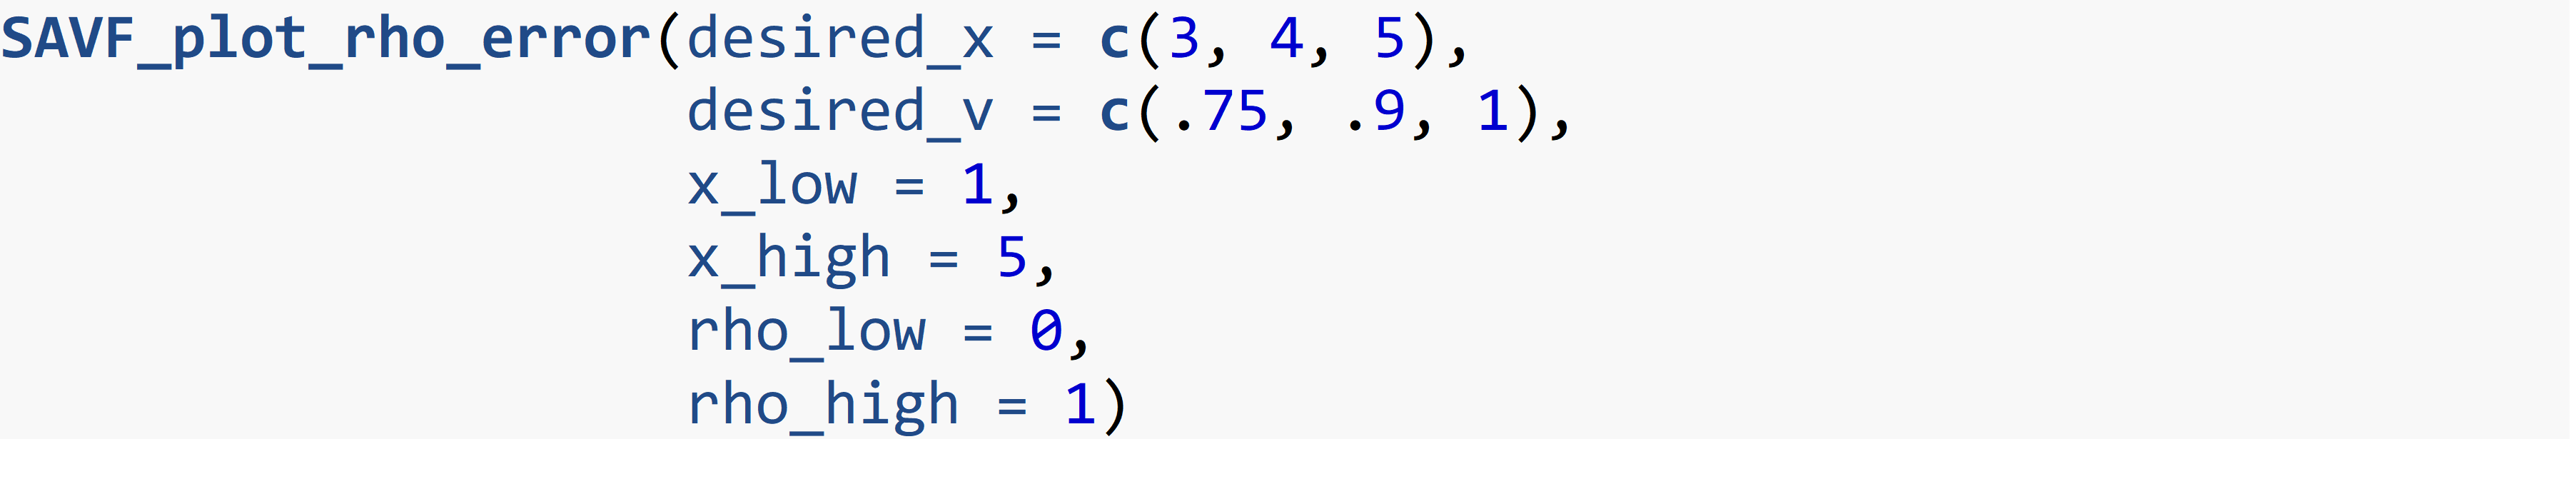
\includegraphics[width=0.5\textwidth]{code7.png}
\end{figure}

\begin{figure}[H]%[!htb]
  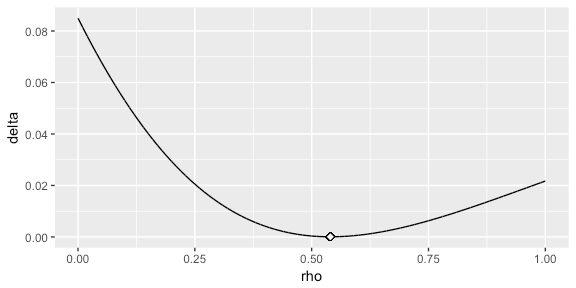
\includegraphics[width=0.5\textwidth]{fig4.png}
  \caption{Single attribute utility error curve.}
  \label{fig:4}
\end{figure}

Once we've identified the preferred $\rho$ value, we can now apply the exponential SAVF with SAVF\_score to normalize our attributes based on our utility curve. Here, we assume that the optimal $\rho$ value for the $x$ and $y$ attributes are 0.653 and 0.70, respectively.
% \begin{Verbatim}[fontsize=\footnotesize]
% library(dplyr)
% 
% psc <- psc %>%
%   mutate(x_SAVF_score = SAVF_score(x_attribute, 1, 5, 0.653),
%          y_SAVF_score = SAVF_score(y_attribute, 1, 10, 0.70))
% 
% psc
% ## # A tibble: 200 x 5
% ##      PSC x_attribute y_attribute x_SAVF_score y_SAVF_score
% ##    <chr>       <dbl>       <dbl>        <dbl>        <dbl>
% ## 1   D233        3.01        4.84    0.7887459    0.9336977
% ## 2   F352        4.34        5.64    0.9573299    0.9629164
% ## 3   T713        3.37        4.30    0.8495938    0.9023958
% ## 4   K833        2.67        5.53    0.7165401    0.9598009
% ## 5   Q121        3.48        4.33    0.8655080    0.9044624
% ## 6   C791        3.32        7.32    0.8419735    0.9898314
% ## 7   Y207        3.48        5.42    0.8655080    0.9564360
% ## 8   W439        2.47        3.35    0.6659448    0.8084720
% ## 9   N290        1.66        4.02    0.3778582    0.8808636
% ## 10  C251        1.00        7.47    0.0000000    0.9910284
% ## # ... with 190 more rows
% \end{Verbatim}
\begin{figure}[!htb]
  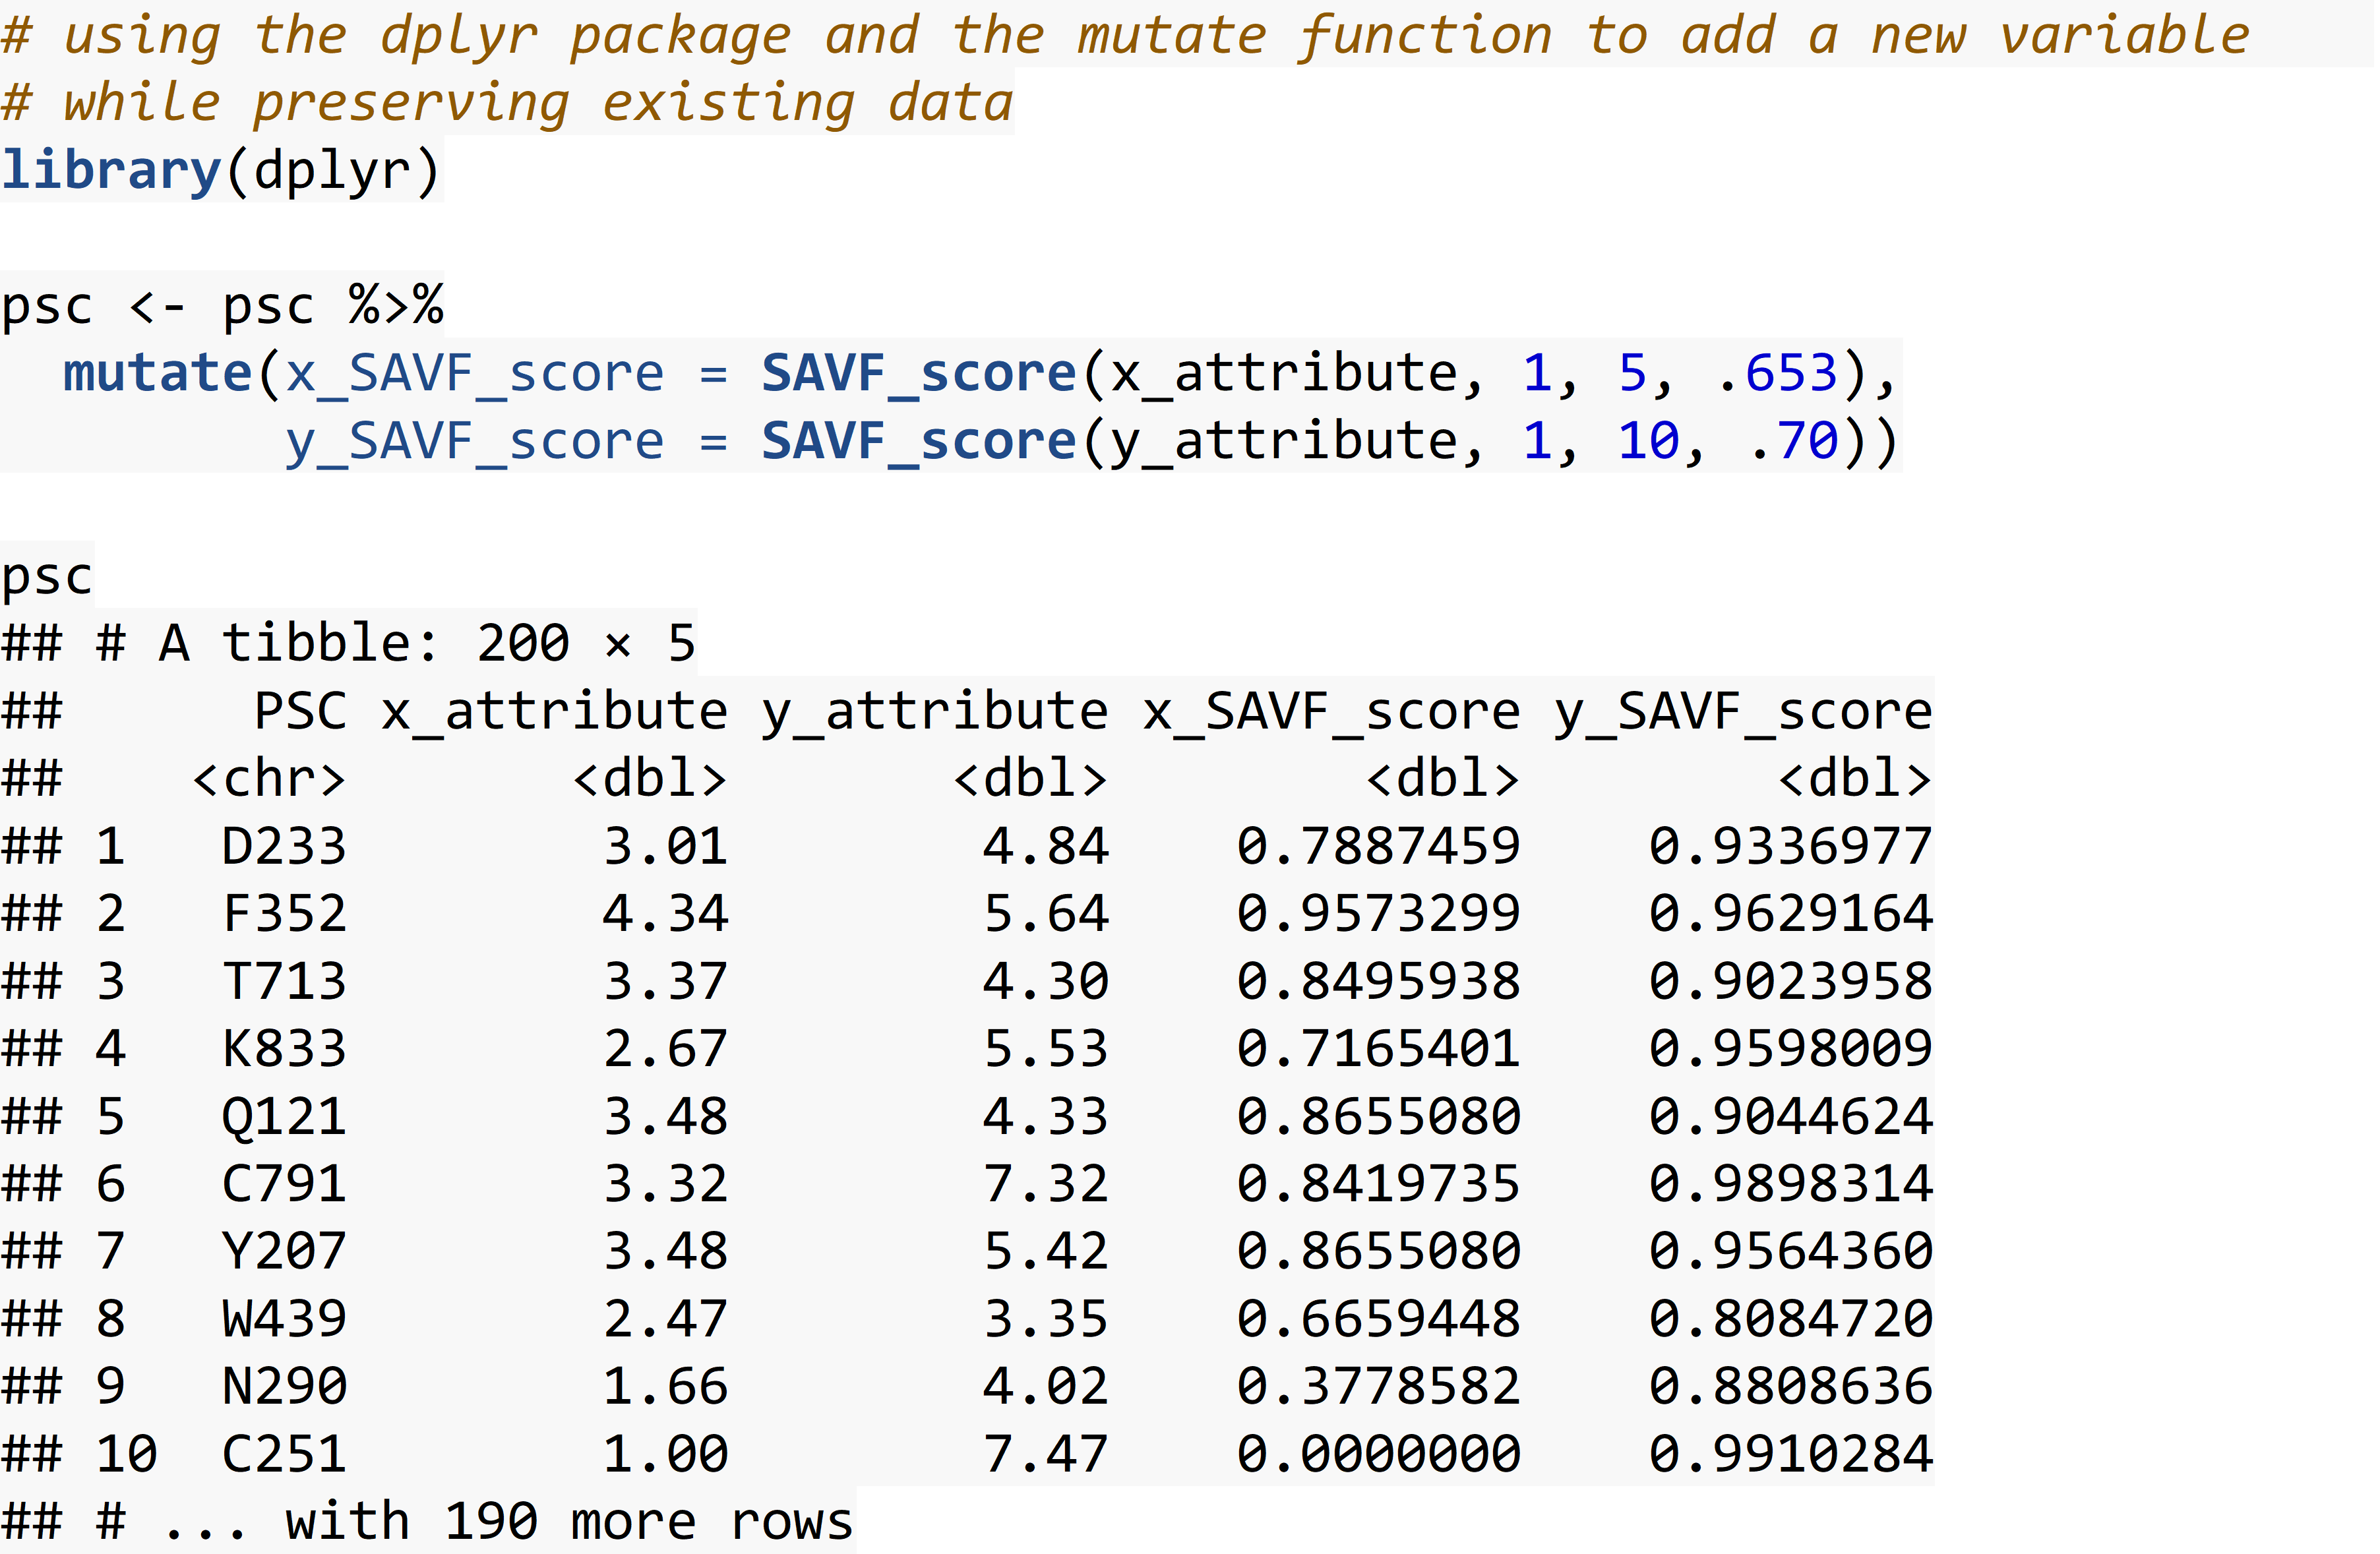
\includegraphics[width=0.5\textwidth]{code8.png}
\end{figure}

Now that we have the normalized $x$ and $y$ attribute utility scores that align to our leadership's preference structure, we can proceed with plotting each PSC within the Kraljic matrix with the kraljic\_matrix function.
% \begin{Verbatim}[fontsize=\footnotesize]
% kraljic_matrix(psc, x_SAVF_score, y_SAVF_score)
% \end{Verbatim}
\begin{figure}[!htb]
  
\includegraphics[width=0.5\textwidth]{code9.png}
\end{figure}

\begin{figure}[!htb]
  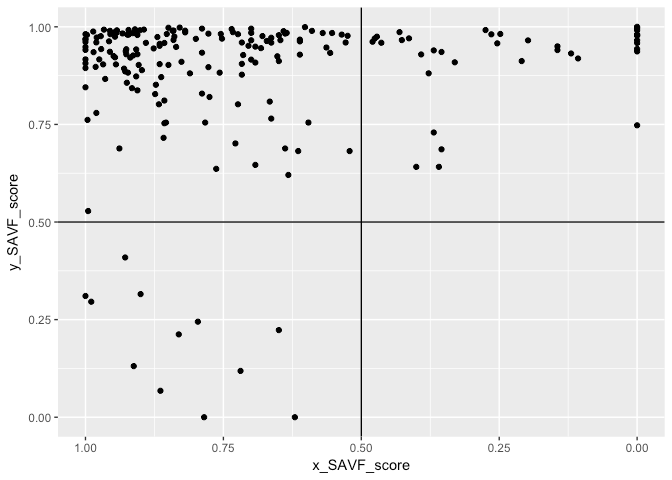
\includegraphics[width=0.5\textwidth]{fig5.png}
  \caption{kraljic\_matrix function output.}
  \label{fig:5}
\end{figure}

This illustrates that most of our PSCs fall in the "Leverage" (upper left) quadrant while a few fall in the "Strategic" (upper right) and "Non-critical" (lower left) quadrants and no PSCs fall in the "Bottleneck" quadrant. Keep in mind that each category benefits from a different strategic sourcing approach. Consequently, decision-makers benefit from understanding specifically which products and services align to each so that they can coordinate the appropriate sourcing strategy for that particular product or service. We can easily do this with the kraljic\_quadrant function.
% \begin{Verbatim}[fontsize=\footnotesize]
% psc %>%
%   mutate(quadrant = kraljic_quadrant(x_SAVF_score, y_SAVF_score))
% ## # A tibble: 200 x 6
% ##      PSC x_attribute y_attribute x_SAVF_score y_SAVF_score  quadrant
% ##    <chr>       <dbl>       <dbl>        <dbl>        <dbl>     <chr>
% ## 1   D233        3.01        4.84    0.7887459    0.9336977  Leverage
% ## 2   F352        4.34        5.64    0.9573299    0.9629164  Leverage
% ## 3   T713        3.37        4.30    0.8495938    0.9023958  Leverage
% ## 4   K833        2.67        5.53    0.7165401    0.9598009  Leverage
% ## 5   Q121        3.48        4.33    0.8655080    0.9044624  Leverage
% ## 6   C791        3.32        7.32    0.8419735    0.9898314  Leverage
% ## 7   Y207        3.48        5.42    0.8655080    0.9564360  Leverage
% ## 8   W439        2.47        3.35    0.6659448    0.8084720  Leverage
% ## 9   N290        1.66        4.02    0.3778582    0.8808636 Strategic
% ## 10  C251        1.00        7.47    0.0000000    0.9910284 Strategic
% ## # ... with 190 more rows
% \end{Verbatim}
\begin{figure}[!htb]
  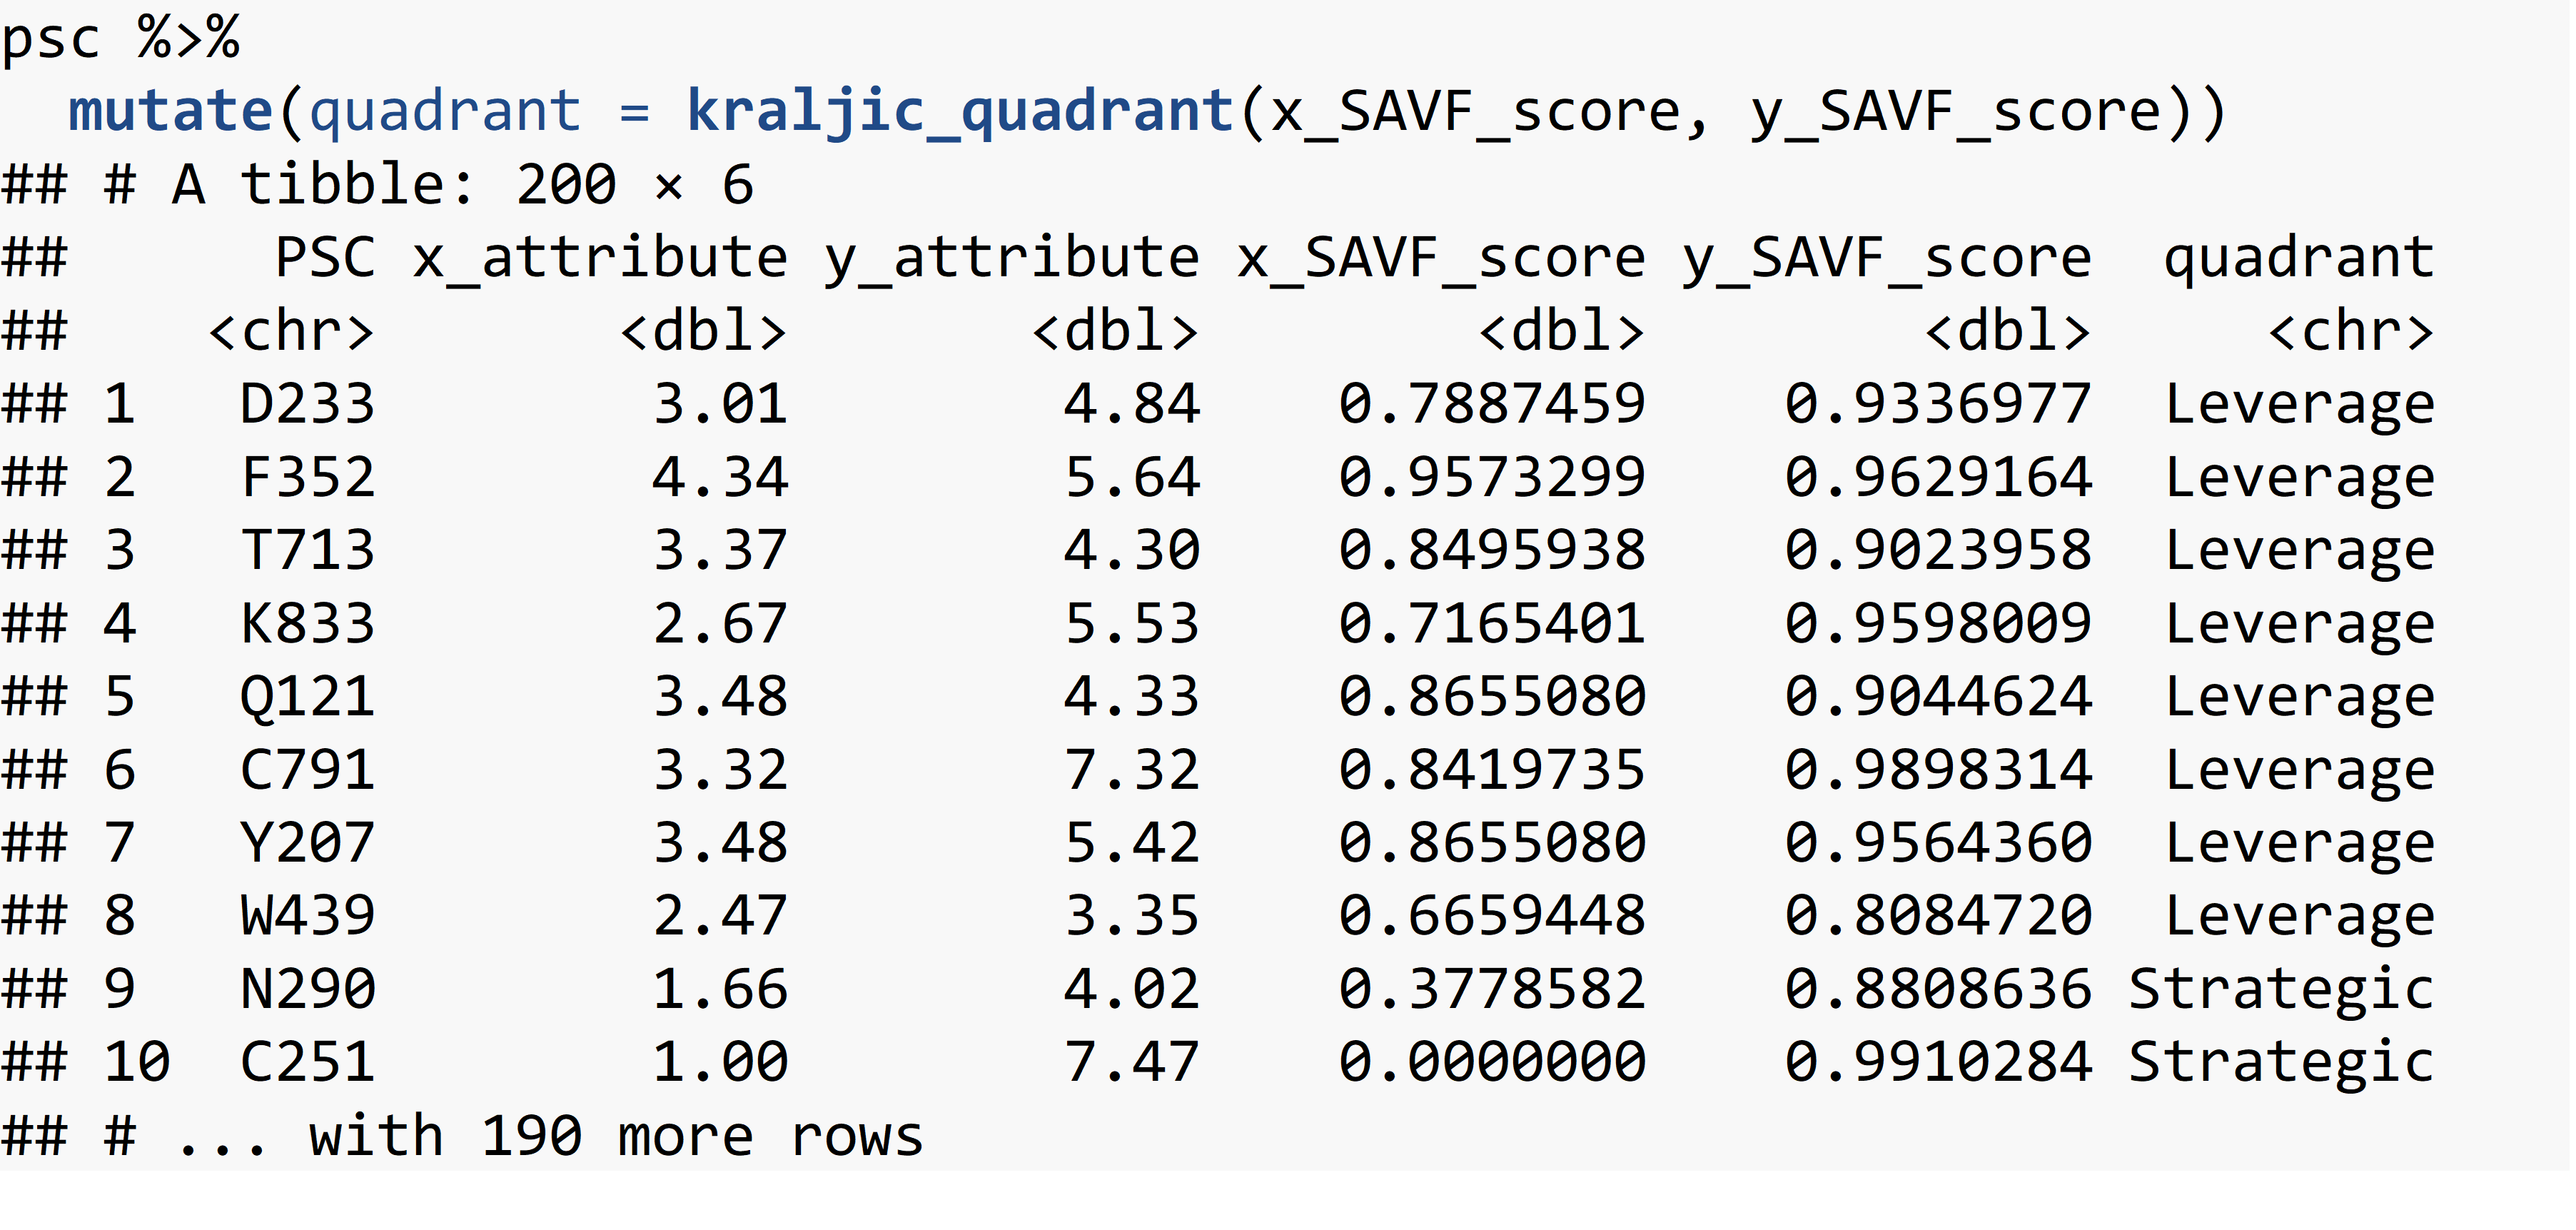
\includegraphics[width=0.5\textwidth]{code10.png}
\end{figure}
An analyst can now easily filter for those PSCs that fall in a specific quadrant.  Lastly, it is important to keep in mind that decision-makers may weight the importance of each attribute differently. Due to certain market environments, decision-makers may weight the $x$ attribute (i.e., supply risk) of greater importance than the $y$ attribute (i.e., profit impact) or vice versa.  One approach used in the extant literature is importance weighting (i.e., see \citet{oe97,lx08,pwa12}.  However, importance weights do not take into account the range between the least- and most-preferred options on each attribute (see Winterfeldt and Edwards, 1993).  Rather, swing weighting has become a common approach to more accurately capture the importance trade-space of given attributes \citep{pbtj13}. There is a unique difference between importance weighting and swing weighting. "Importance weights are used to reflect the general importance of one attribute over another...without regard to...the difference between the worst and the best value points of each attribute" \citep[p. 200]{wb87}. Watson and Buede further state that "when this difference from worst to best is not explicitly referenced in assessing weights, we obtain some general notion of importance, which is subject to great variation and argument among decision-makers" \citep[p. 200]{wb87}. \citet{dpbhc08} argue that "importance weights do not take into account the range between the lowest and the highest levels of the value measures" resulting in the potential for important measures to not be important to the decision. Keeney (2009) adds that "when we quantify objectives by simply asking for their relative importance, considerable misinformation about values is produced and a substantial opportunity to understand values is lost."  However, the use of swing weighting ensures we capture the full value preference structure rather than simply an arbitrary score or at best a hierarchy of importance. Swing weighting also protects against the potential for loss of information, misunderstanding of decision-maker belief, and even loss of trade-offs between values.  Thus, we can prioritize PSCs based on this preference by applying a multi-attribute value function (MAVF) with swing weights. Swing weight values for $x$ and $y$ attributes ($w_x$ and $w_y$ respectively) are typically elicited from SMEs (for a detailed description of this process see von Winterfeldt and Edwards, 1993). This allows for calculation of the interaction swing weight $w_{xy} = 1 - w_x - w_y$. Thus, we can calculate the MAVF as outlined by \citet{kr93}:
\begin{equation}
\label{eqn:2}
V\left(x, y\right) = w_x v_x\left(x\right) + w_y v_y\left(y\right) + w_{xy} v_x\left(x\right)v_y\left(y\right).
\end{equation}

We can apply the MAVF\_score function to compute the multi-attribute value score based on $x$ and $y$ attribute utility scores and their respective swing weights. Hence, if through discussions with decision-makers we identify swing weight values of 0.65 and 0.35 for the $x$ and $y$ attributes respectively, we can obtain the computed MAVF score for each PSC:

% \begin{Verbatim}[fontsize=\footnotesize]
% psc %>%
%   mutate(MAVF = MAVF_score(x_SAVF_score, y_SAVF_score, 0.65, 0.35))
% ## # A tibble: 200 x 6
% ##      PSC x_attribute y_attribute x_SAVF_score y_SAVF_score      MAVF
% ##    <chr>       <dbl>       <dbl>        <dbl>        <dbl>     <dbl>
% ## 1   D233        3.01        4.84    0.7887459    0.9336977 0.8394790
% ## 2   F352        4.34        5.64    0.9573299    0.9629164 0.9592852
% ## 3   T713        3.37        4.30    0.8495938    0.9023958 0.8680745
% ## 4   K833        2.67        5.53    0.7165401    0.9598009 0.8016814
% ## 5   Q121        3.48        4.33    0.8655080    0.9044624 0.8791420
% ## 6   C791        3.32        7.32    0.8419735    0.9898314 0.8937237
% ## 7   Y207        3.48        5.42    0.8655080    0.9564360 0.8973328
% ## 8   W439        2.47        3.35    0.6659448    0.8084720 0.7158293
% ## 9   N290        1.66        4.02    0.3778582    0.8808636 0.5539101
% ## 10  C251        1.00        7.47    0.0000000    0.9910284 0.3468599
% ## # ... with 190 more rows
% \end{Verbatim}
\begin{figure}[!htb]
  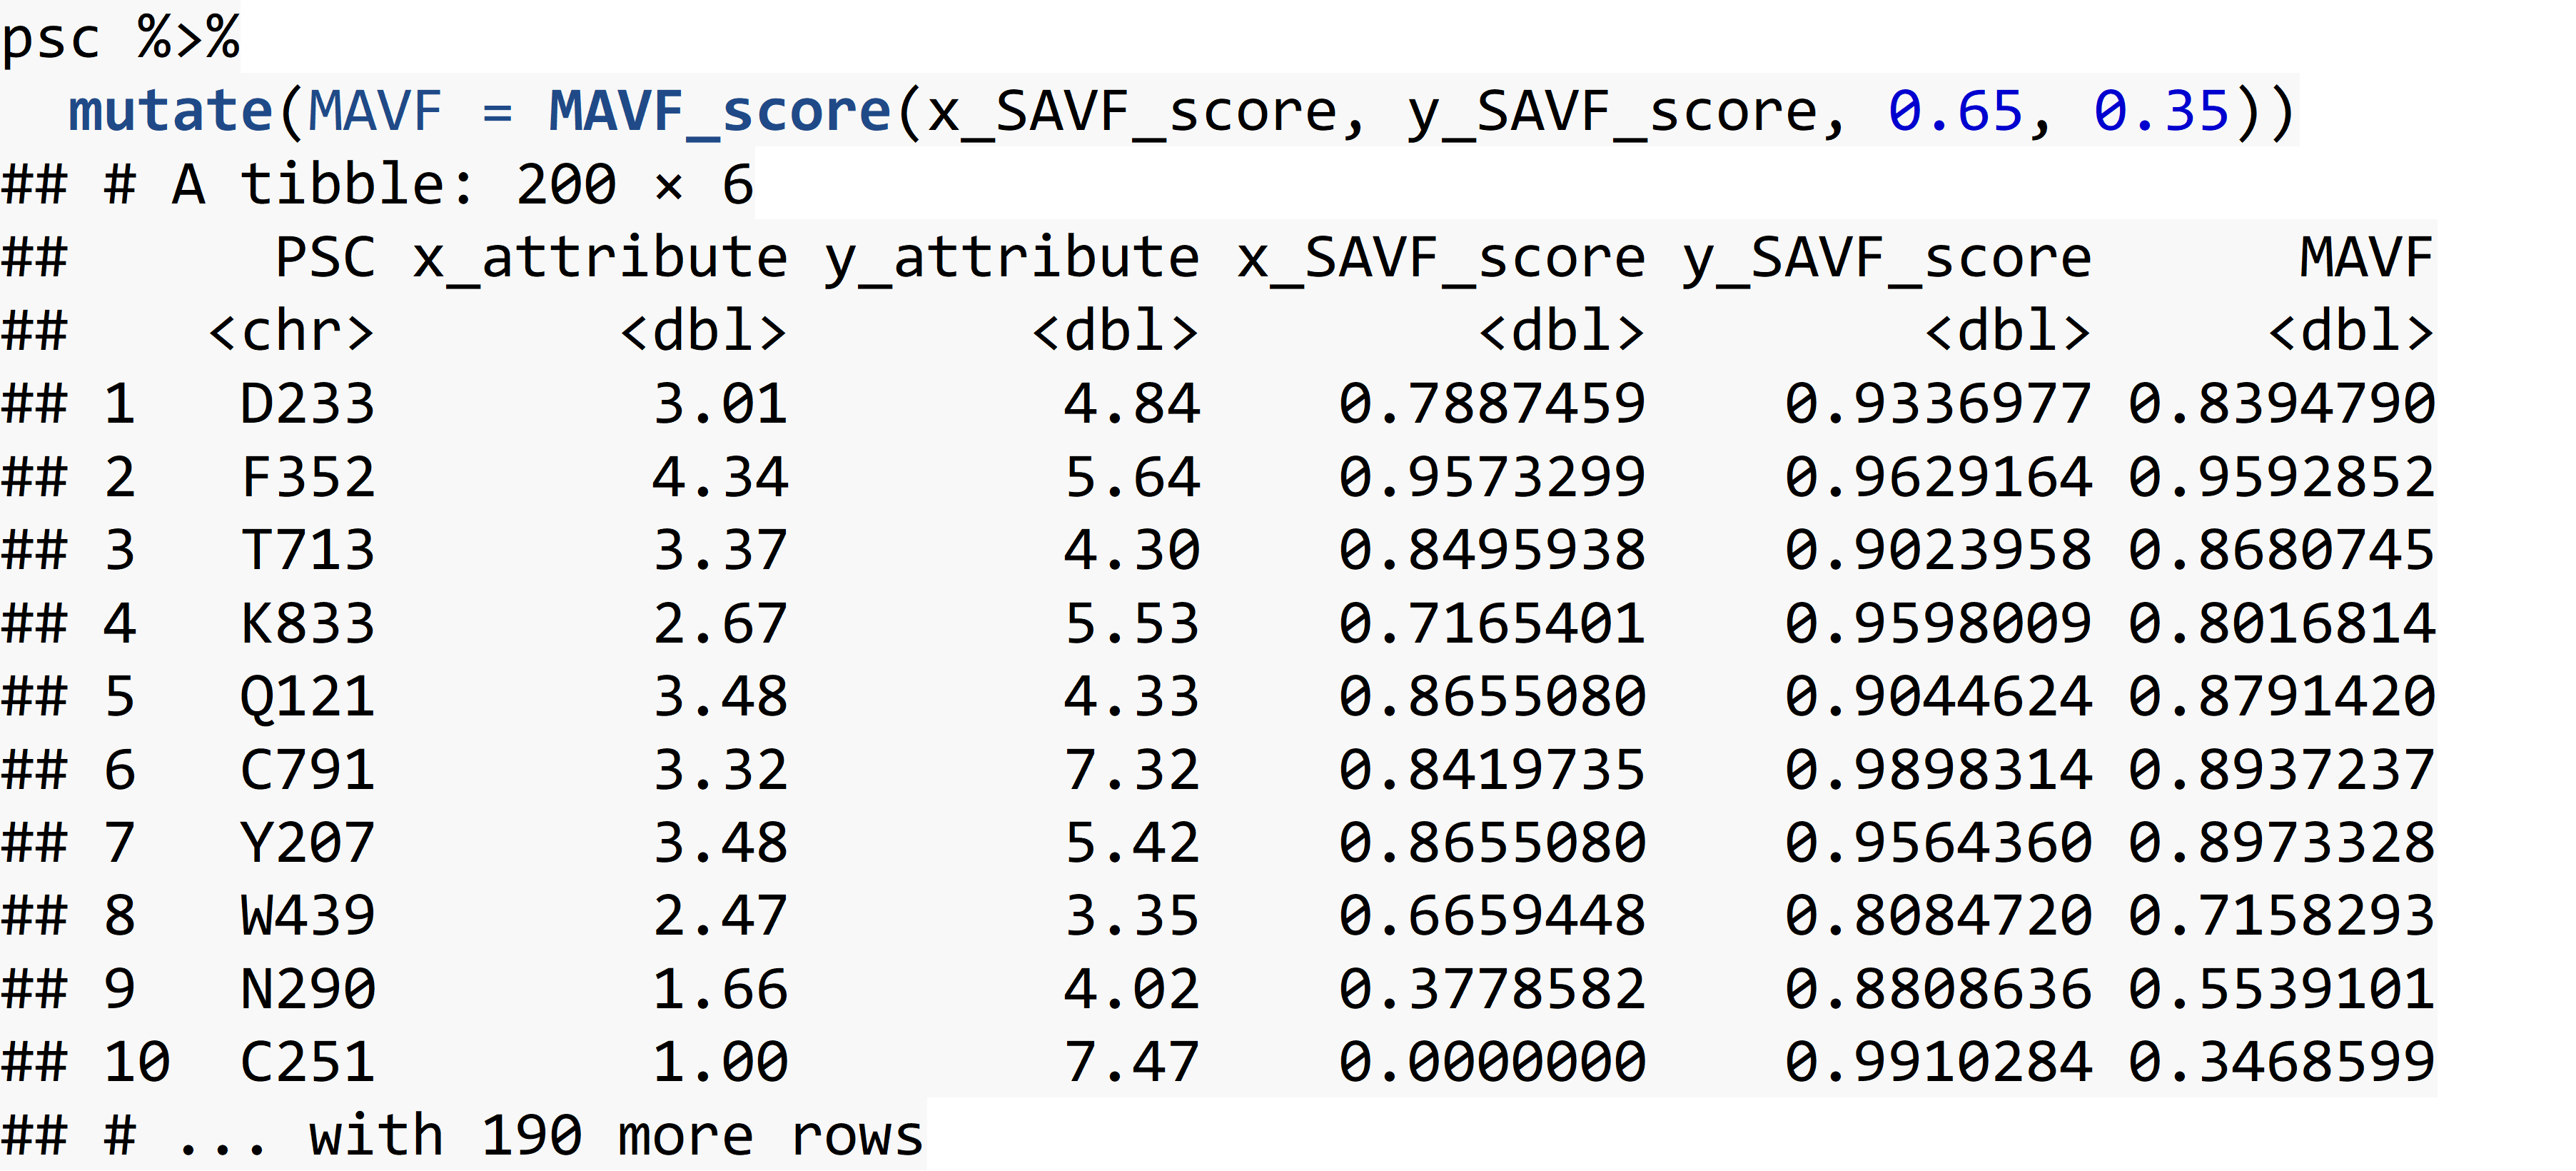
\includegraphics[width=0.5\textwidth]{code11.png}
\end{figure}

This allows us to quickly dissect our PSCs. For example, if decision-makers are most concerned with the "Leverage" quadrant but want to assess the top 10 PSCs based on the decision-makers preferences of the attributes, we can efficiently make this assessment with the following code. This identifies the top 10 PSCs that are most likely to benefit from a strategic sourcing approach specifically designed for "Leverage" PSCs.
% \begin{Verbatim}[fontsize=\footnotesize]
% psc %>%
%   mutate(MAVF = MAVF_score(x_SAVF_score, y_SAVF_score, 0.65, 0.35),
%          quadrant = kraljic_quadrant(x_SAVF_score, y_SAVF_score)) %>%
%   filter(quadrant == "Leverage") %>%
%   top_n(10, wt = MAVF)
% ## # A tibble: 10 x 7
% ##      PSC x_attribute y_attribute x_SAVF_score y_SAVF_score      MAVF
% ##    <chr>       <dbl>       <dbl>        <dbl>        <dbl>     <dbl>
% ## 1   Y357        5.00        6.55    1.0000000    0.9812541 0.9934389
% ## 2   E103        4.46        7.71    0.9665150    0.9927003 0.9756799
% ## 3   C432        4.65        6.05    0.9796633    0.9726273 0.9772007
% ## 4   P402        5.00        5.82    1.0000000    0.9675243 0.9886335
% ## 5   Q255        4.95        6.41    0.9973714    0.9791345 0.9909885
% ## 6   H426        5.00        5.58    1.0000000    0.9612468 0.9864364
% ## 7   E908        4.75        7.11    0.9859554    0.9879299 0.9866465
% ## 8   X634        5.00        5.19    1.0000000    0.9485047 0.9819766
% ## 9   O288        5.00        5.00    1.0000000    0.9409177 0.9793212
% ## 10  V870        5.00        5.88    1.0000000    0.9689357 0.9891275
% ## # ... with 1 more variables: quadrant <chr>
% \end{Verbatim}
\begin{figure}[!htb]
  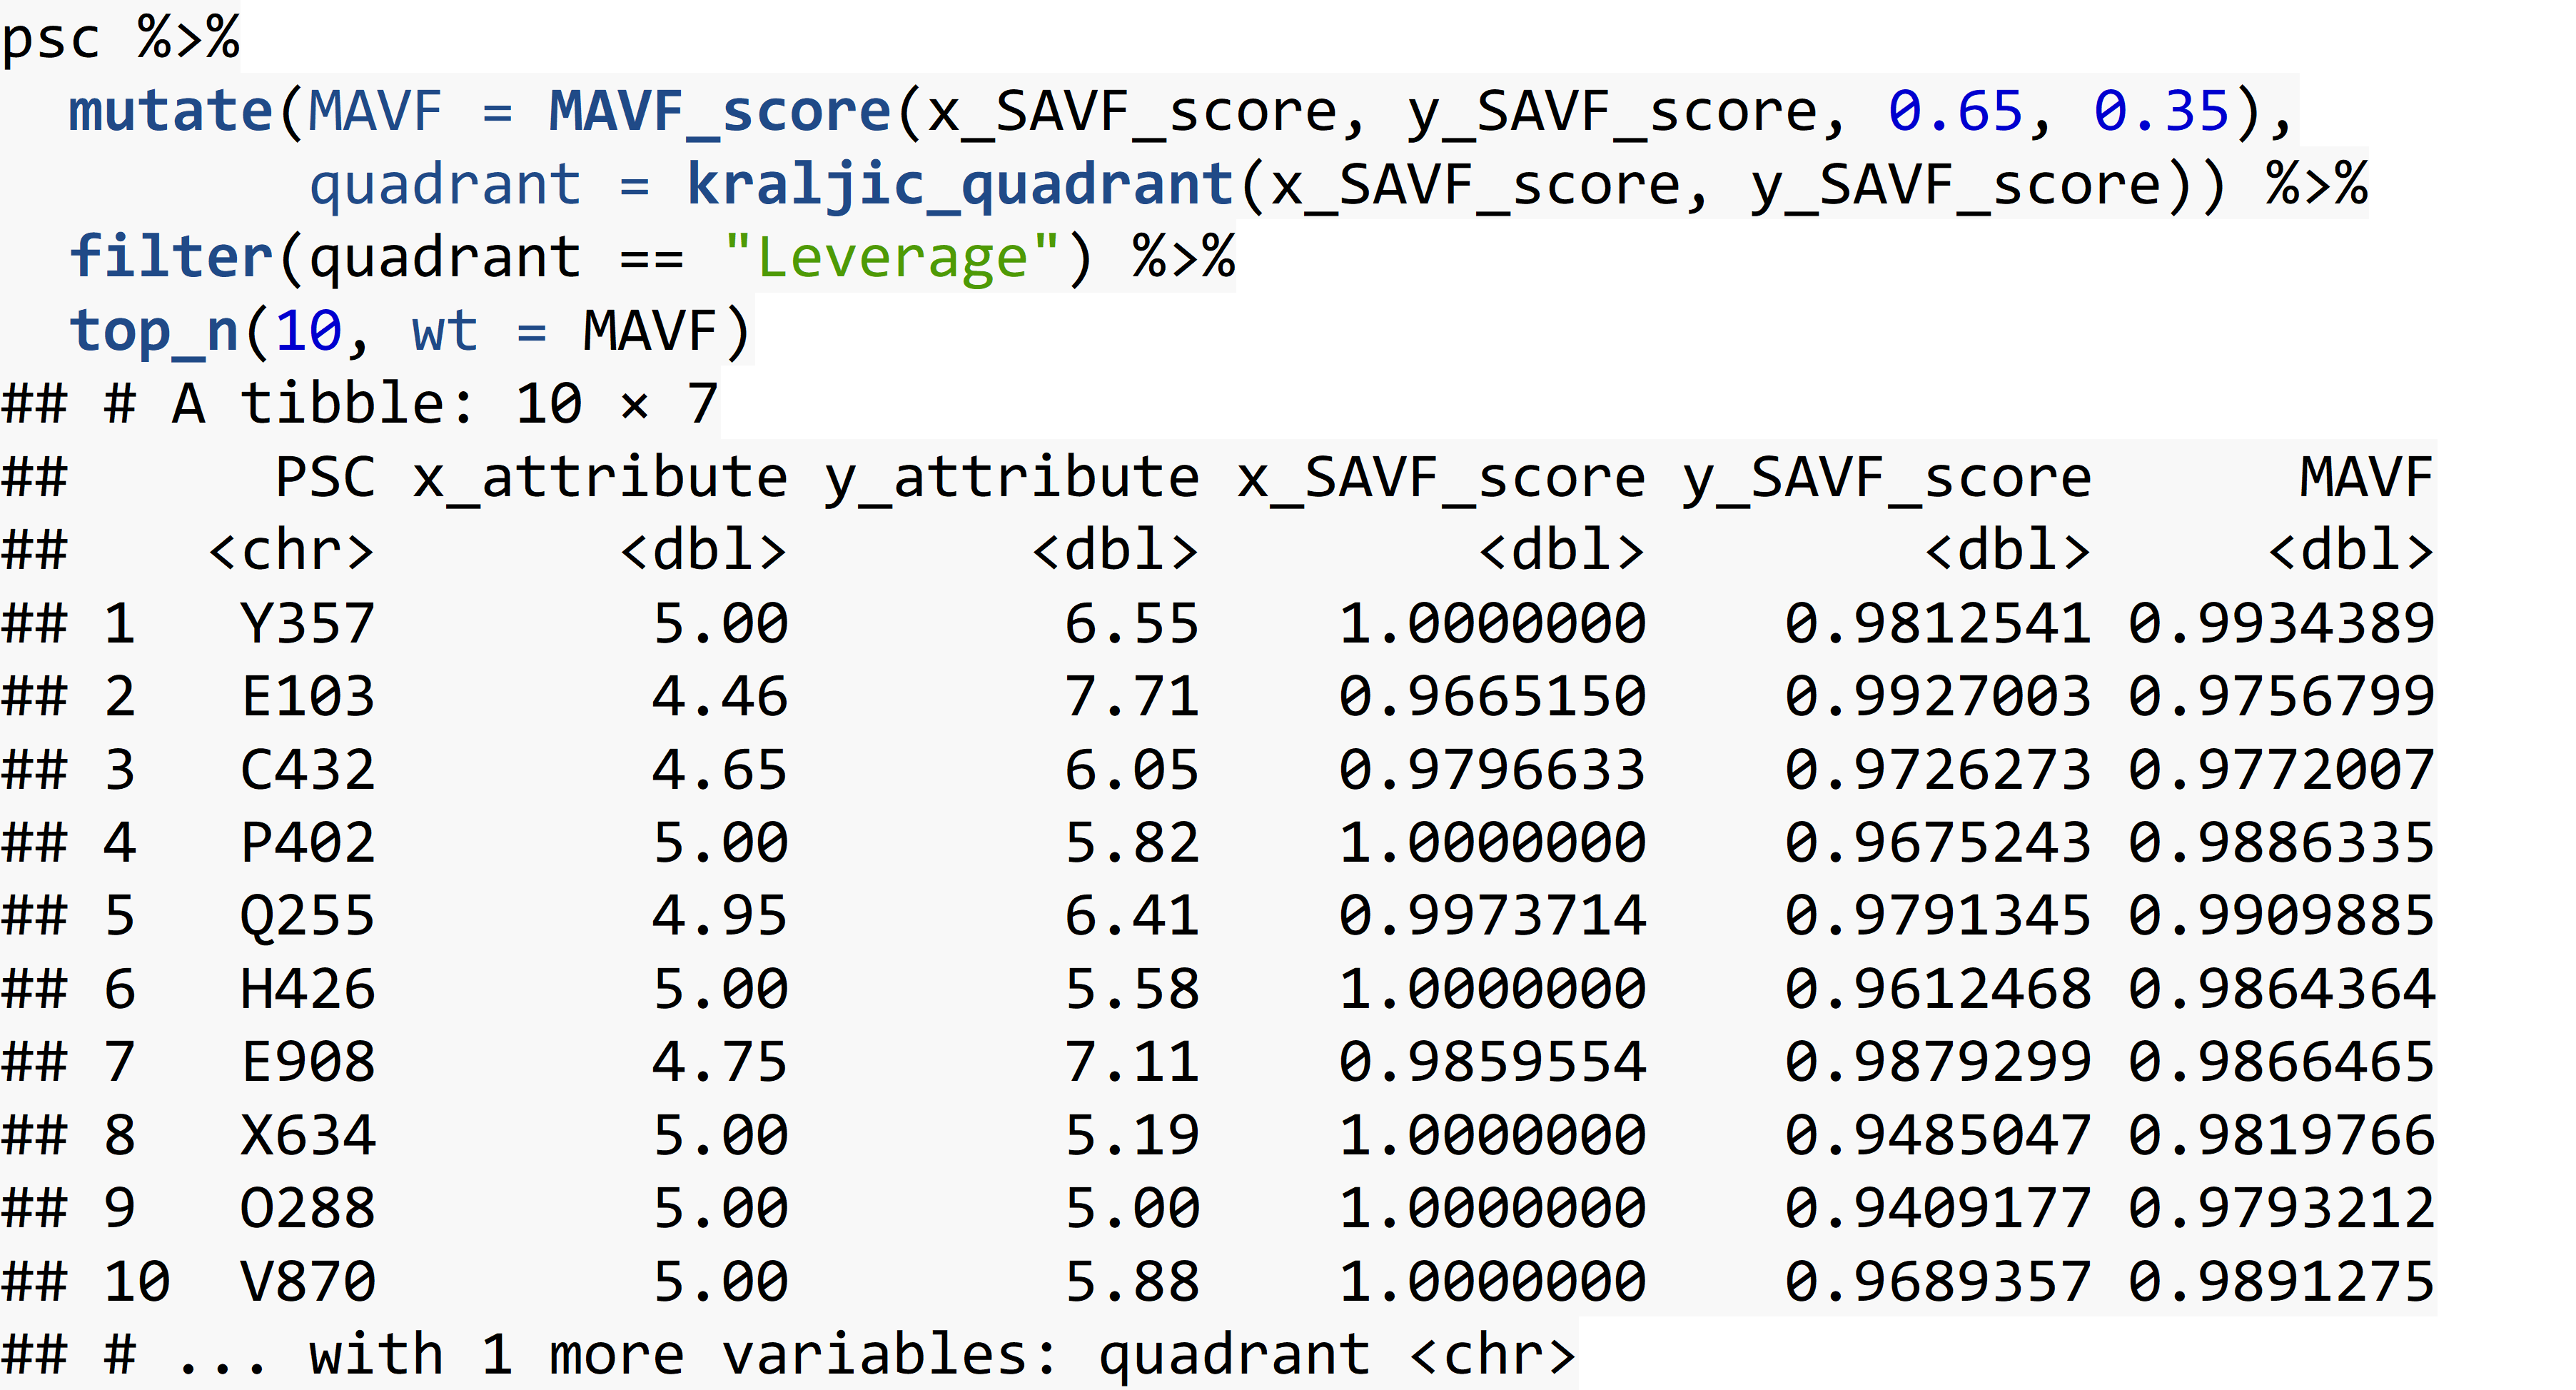
\includegraphics[width=0.5\textwidth]{code12.png}
\end{figure}

And finally, since our swing weight inputs are subjective in nature, we may wish to perform a sensitivity analysis on these swing weights to see their impact on MAVF scores. The MAVF\_sensitivity function executes a sensitivity analysis by performing a Monte Carlo simulation with 1000 trials for each product or service (row). Each trial randomly selects a weight from a uniform distribution between lower and upper bound swing weight parameters and calculates the multi-attribute utility score. From these trials, summary statistics for each product or service (row) are calculated and reported for the final output. 
% \begin{Verbatim}[fontsize=\footnotesize]
% MAVF_sensitivity(psc,
%                  x = x_SAVF_score,
%                  y = y_SAVF_score,
%                  x_wt_min = 0.55,
%                  x_wt_max = 0.75,
%                  y_wt_min = 0.25,
%                  y_wt_max = 0.45) %>%
%   select(PSC, starts_with("MAVF"))
% ## # A tibble: 200 x 8
% ##      PSC MAVF_Min MAVF_1st_Q MAVF_Median MAVF_Mean MAVF_3rd_Q MAVF_Max
% ##    <chr>    <dbl>      <dbl>       <dbl>     <dbl>      <dbl>    <dbl>
% ## 1   D233   0.8148     0.8294      0.8390    0.8392     0.8489   0.8636
% ## 2   F352   0.9517     0.9569      0.9590    0.9592     0.9614   0.9667
% ## 3   T713   0.8465     0.8609      0.8676    0.8678     0.8744   0.8891
% ## 4   K833   0.7718     0.7881      0.8003    0.8013     0.8151   0.8311
% ## 5   Q121   0.8590     0.8726      0.8786    0.8789     0.8850   0.8988
% ## 6   C791   0.8774     0.8859      0.8928    0.8935     0.9016   0.9099
% ## 7   Y207   0.8809     0.8907      0.8970    0.8971     0.9035   0.9134
% ## 8   W439   0.6765     0.7017      0.7151    0.7153     0.7285   0.7542
% ## 9   N290   0.4951     0.5264      0.5510    0.5532     0.5813   0.6120
% ## 10  C251   0.2480     0.2979      0.3414    0.3456     0.3958   0.4458
% ## # ... with 190 more rows, and 1 more variables: MAVF_Range <dbl>
% \end{Verbatim}
\begin{figure}[!htb]
  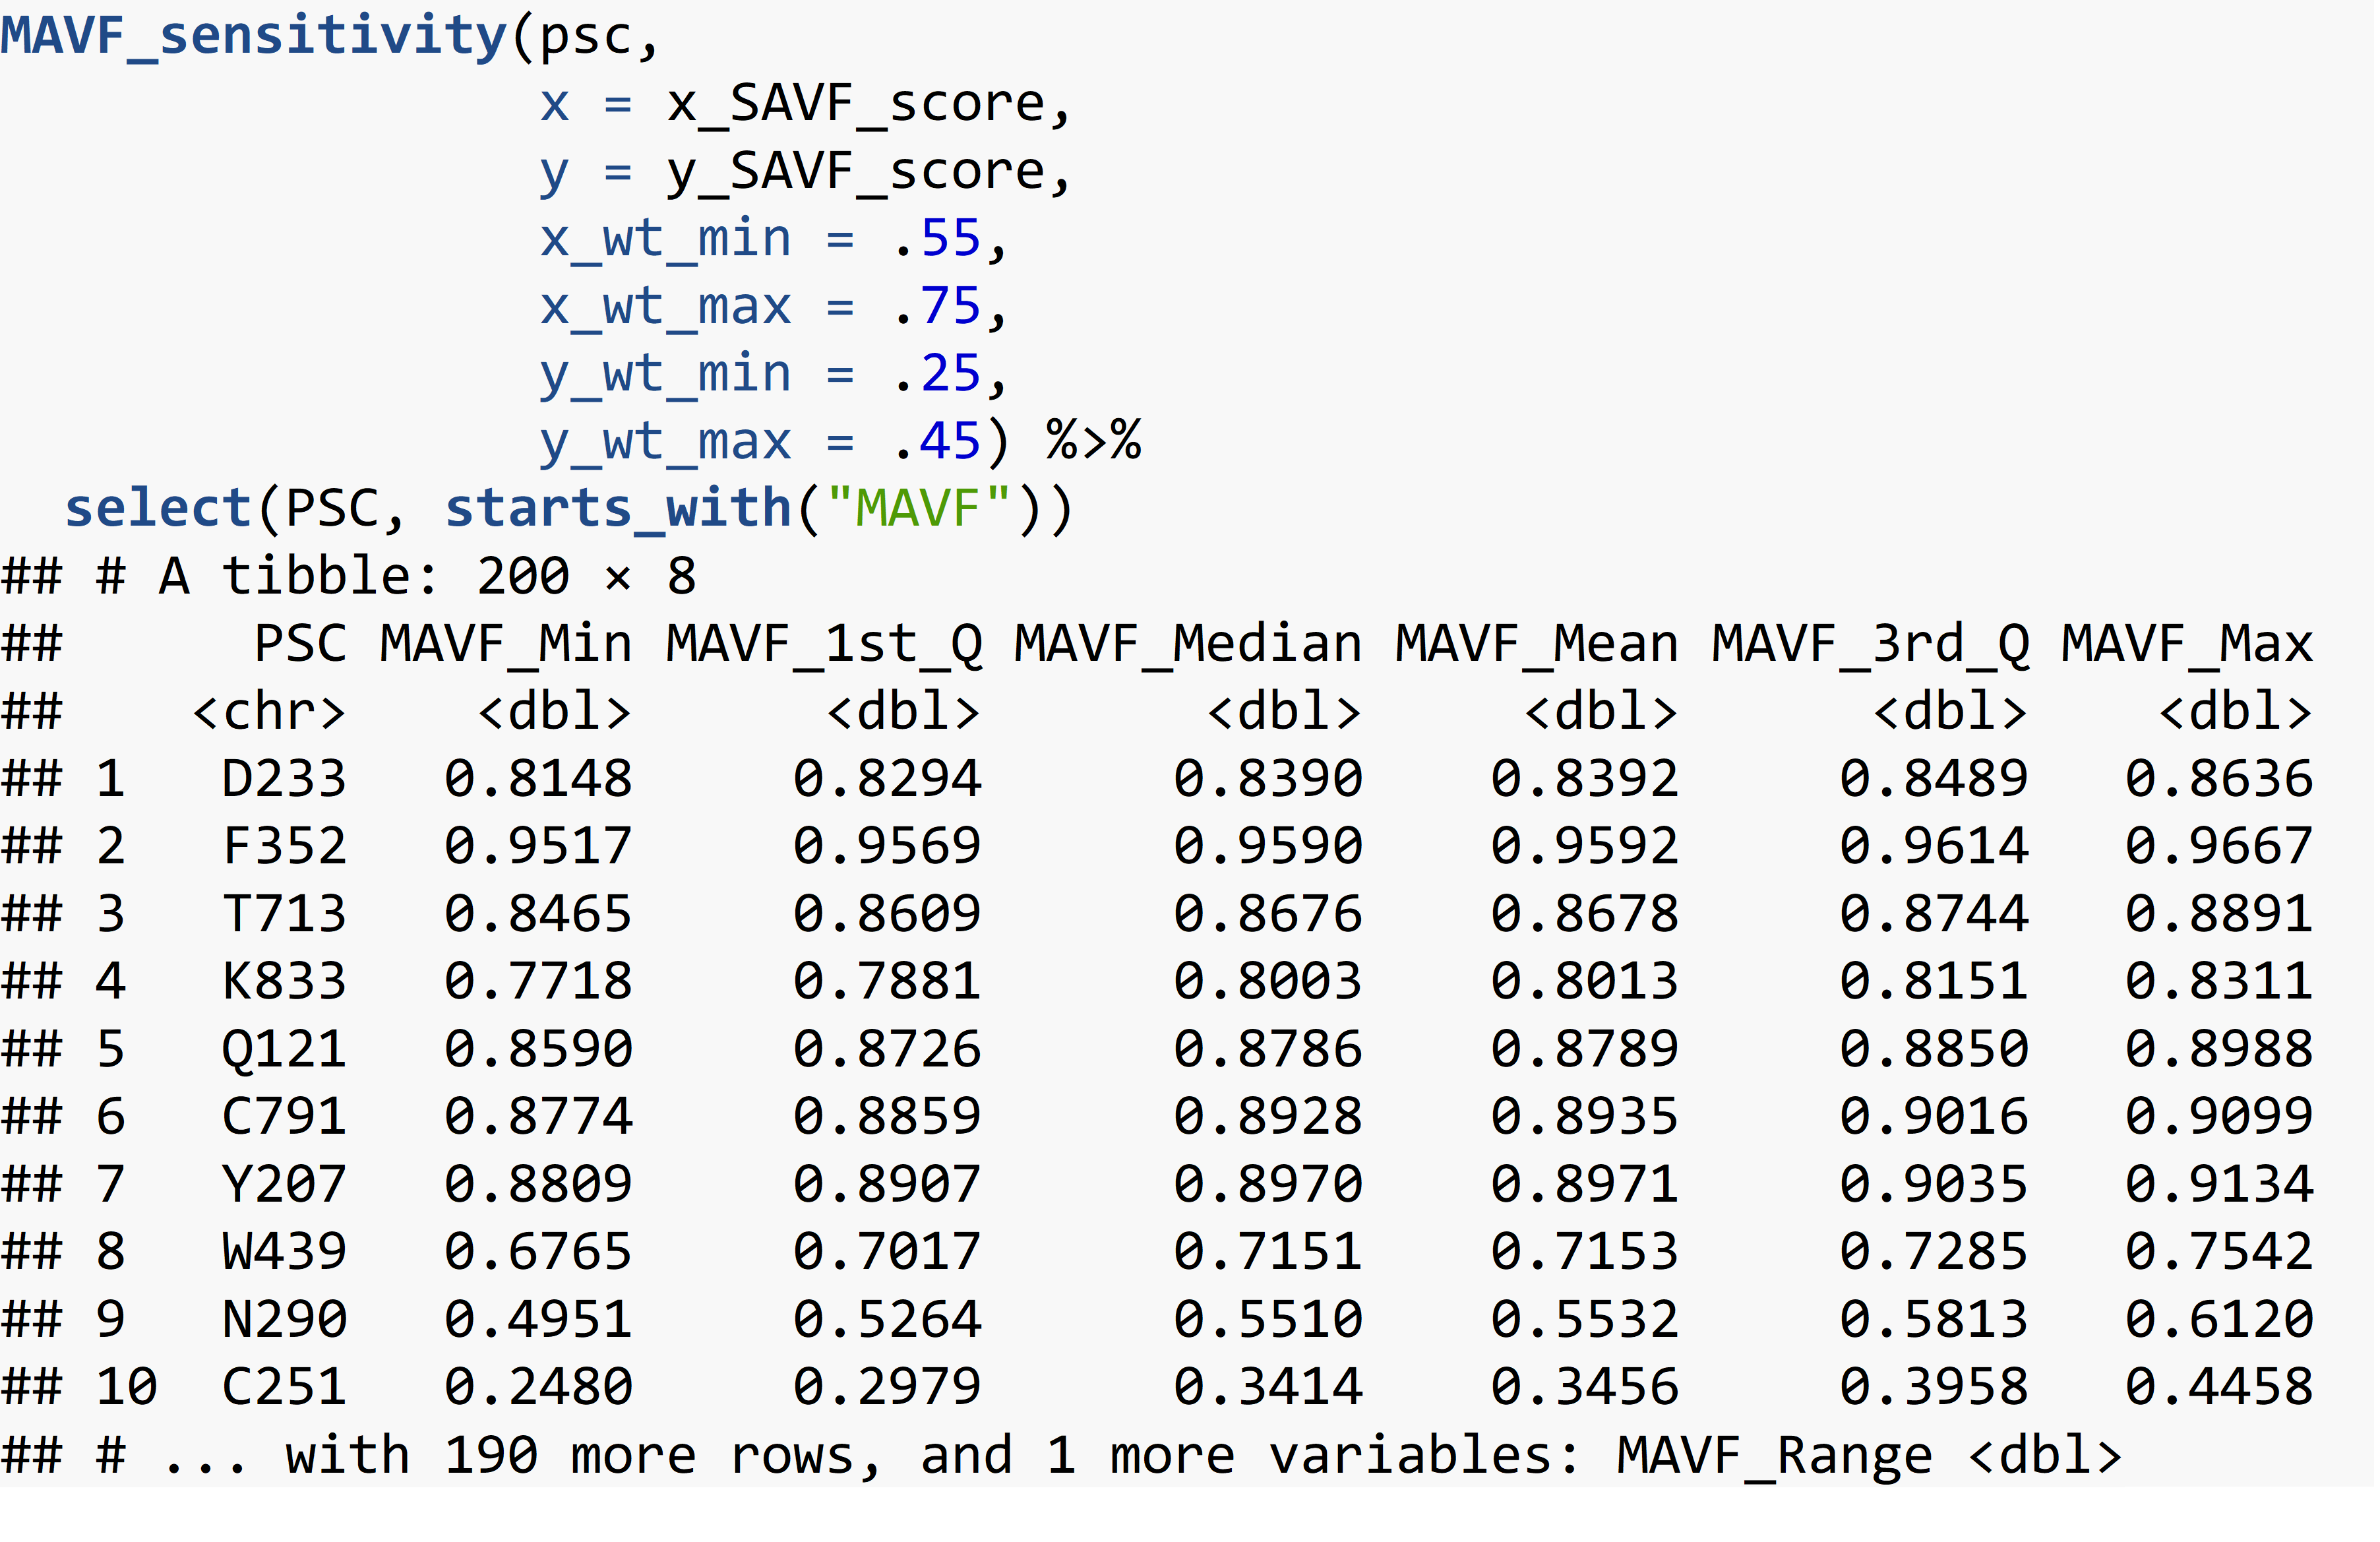
\includegraphics[width=0.5\textwidth]{code13.png}
\end{figure}

Although this provides the basic understanding of each KraljicMatrix function, additional information can be found for each function by running ?function (i.e., ?SAVF\_score).  Next, we'll illustrate an operationalization of the KraljicMatrix package. 


%%%%%%%%%%%%%%%%%%%%%%%%%%%%%%%%%%%%%%%%%%%%%%%%%%%%%%%%%%%%%%%%%%%%%%%%%%%%%%%%
\section{Case Exemplar: A Practical Operationalization of the KraljicMatrix Package}
\label{sec:5}
%%%%%%%%%%%%%%%%%%%%%%%%%%%%%%%%%%%%%%%%%%%%%%%%%%%%%%%%%%%%%%%%%%%%%%%%%%%%%%%%


%%%%%%%%%%%%%%%%%%%%%%%%%%%%%%%%%%%%%%%%%%%%%%%%%%%%%%%%%%%%%%%%%%%%%%%%%%%%%%%%
\subsection{Background}
\label{sec:5.1}
%%%%%%%%%%%%%%%%%%%%%%%%%%%%%%%%%%%%%%%%%%%%%%%%%%%%%%%%%%%%%%%%%%%%%%%%%%%%%%%%

A 2012 General Accountability Office \citep{gao} report found that the Department of Defense (DoD) has leveraged only a fraction of what could potentially be managed and saved through strategic sourcing \citep{gao}.  Furthermore, a follow-on report in 2015 emphasized that by implementing strategic sourcing via a purchasing portfolio framework, the DoD, and its military agencies could more aggressively leverage their buying power and select appropriate sourcing strategies and tactics \citep{gao2}.  The GAO has made it clear that "strategic sourcing of even one percent [at the DoD level] would equate to billions of dollars" \citep{gao}.

%The Air Force Installation Contracting Agency (AFICA) is the U.S. Air Force (USAF) procurement organization designed to leverage its enterprise reach in order to capitalize on strategic sourcing opportunities that will generate savings to the USAF and maximize value to the American taxpayer.  From Fiscal Year (FY) 2010-2014, AFICA obligated nearly $43 Billion in support of USAF installations. This figure represents nearly 11\% of the total FY10-14 USAF budget. As the USAF continues to face ongoing contingency operations in multiple locations, the increased scrutiny by the GAO to improve strategic sourcing, and the looming threat of an overburdened economy, the need to uncover areas ripe for cost reduction cannot be overstated.  Unfortunately, AFICA is constrained by limited analytic resources.  They currently have only one OR analyst position and that analyst is burdened with all the analytic modeling requirements for the AFICA agency.  Thus, the KraljicMatrix package was originally developed to provide AFICA's OR analyst with an efficient means to implement a quantitative technique to position items within the KPM and identify the products and services offering the highest potential for cost reduction through strategic sourcing.


%%%%%%%%%%%%%%%%%%%%%%%%%%%%%%%%%%%%%%%%%%%%%%%%%%%%%%%%%%%%%%%%%%%%%%%%%%%%%%%%
\subsection{Analysis}
\label{sec:5.2}
%%%%%%%%%%%%%%%%%%%%%%%%%%%%%%%%%%%%%%%%%%%%%%%%%%%%%%%%%%%%%%%%%%%%%%%%%%%%%%%%

AFICA used a subset (258) of their 1,702 PSCs.  This subset accounted for 80\% of FY10-14 installation spend.  AFICA determined that the two attributes to measure their PSCs against include Minimize Supply Market Complexity ($x$-axis) and Maximize Installation Mission Impact ($y$-axis).

To evaluate supply market complexity, AFICA used the IBISWorld Buyer Power Score. IBISWorld is a research organization whose reports delve into supply markets for a particular good or service. The IBISWorld Buyer Power Score is comprised of three components: price trends, market structure, and market risk. Factors within the three components are weighted and scored to produce an overall buyer power score, which ranges between 1.00 and 5.00 with increments of 0.01. Some factors include availability of substitutes, market share concentration, and product specialization. Switching costs are also considered. A higher score indicates greater buyer strength and a less complex market. Therefore, let $X$ be the IBISWorld Buyer Power Score.

\textit{Spend} is defined as the dollars obligated by Air Force contracting agencies. AFICA installation spend data shows that sequestration in FY13 invoked budget cuts of approximately 13\%. However, the FY14 budget for installation spend increased by nearly 6\%. This trend was visible at the most aggregate levels (total USAF and total department spend) down to the most disaggregated levels (installation level spend). Working with senior AF leadership, it was identified that installation commanders are free, to an extent, to exercise judgment in purchasing decisions. Consequently, as FY14 budgets increased, the assumption is that installation commanders applied budget increases first to the installation's most critical goods and services. Thus, we leverage this assumption to deduce which PSCs were most critical to the installation mission by identifying those PSCs that experienced the largest post-sequestration rebound in spend. To do so, we calculate the percent change of spend for each PSC from FY13-14. We also calculate overall installation spend over the same period, compute the deviation between the two, and scaled from 0 to 1.  Therefore, let $Y$ be the delta between the overall installation spend slope and PSC spend slope from FY13 to FY14.

Working with AFICA leadership we identified the preference structure for the $X$ and $Y$ variables to be: $v_x\left(\left\{1, 3, 4, 5\right\}\right) = \left\{0.0, 0.8, 0.9, 1.0\right\}$ and $v_y\left(\left\{-2.0, 0.0, 1.0\right\}\right) = \left\{0.0, 0.9, 1.0\right\}$. Therefore, using this information we could identify the preferred $\rho$ values of 0.653 and 0.933 for $v_x\left(x_i\right)$ and $v_y\left(y_i\right)$ with SAVF\_preferred\_rho and as illustrated with the SAVF\_plot and SAVF\_plot\_rho\_error outputs below.

\begin{figure}[!htb]
  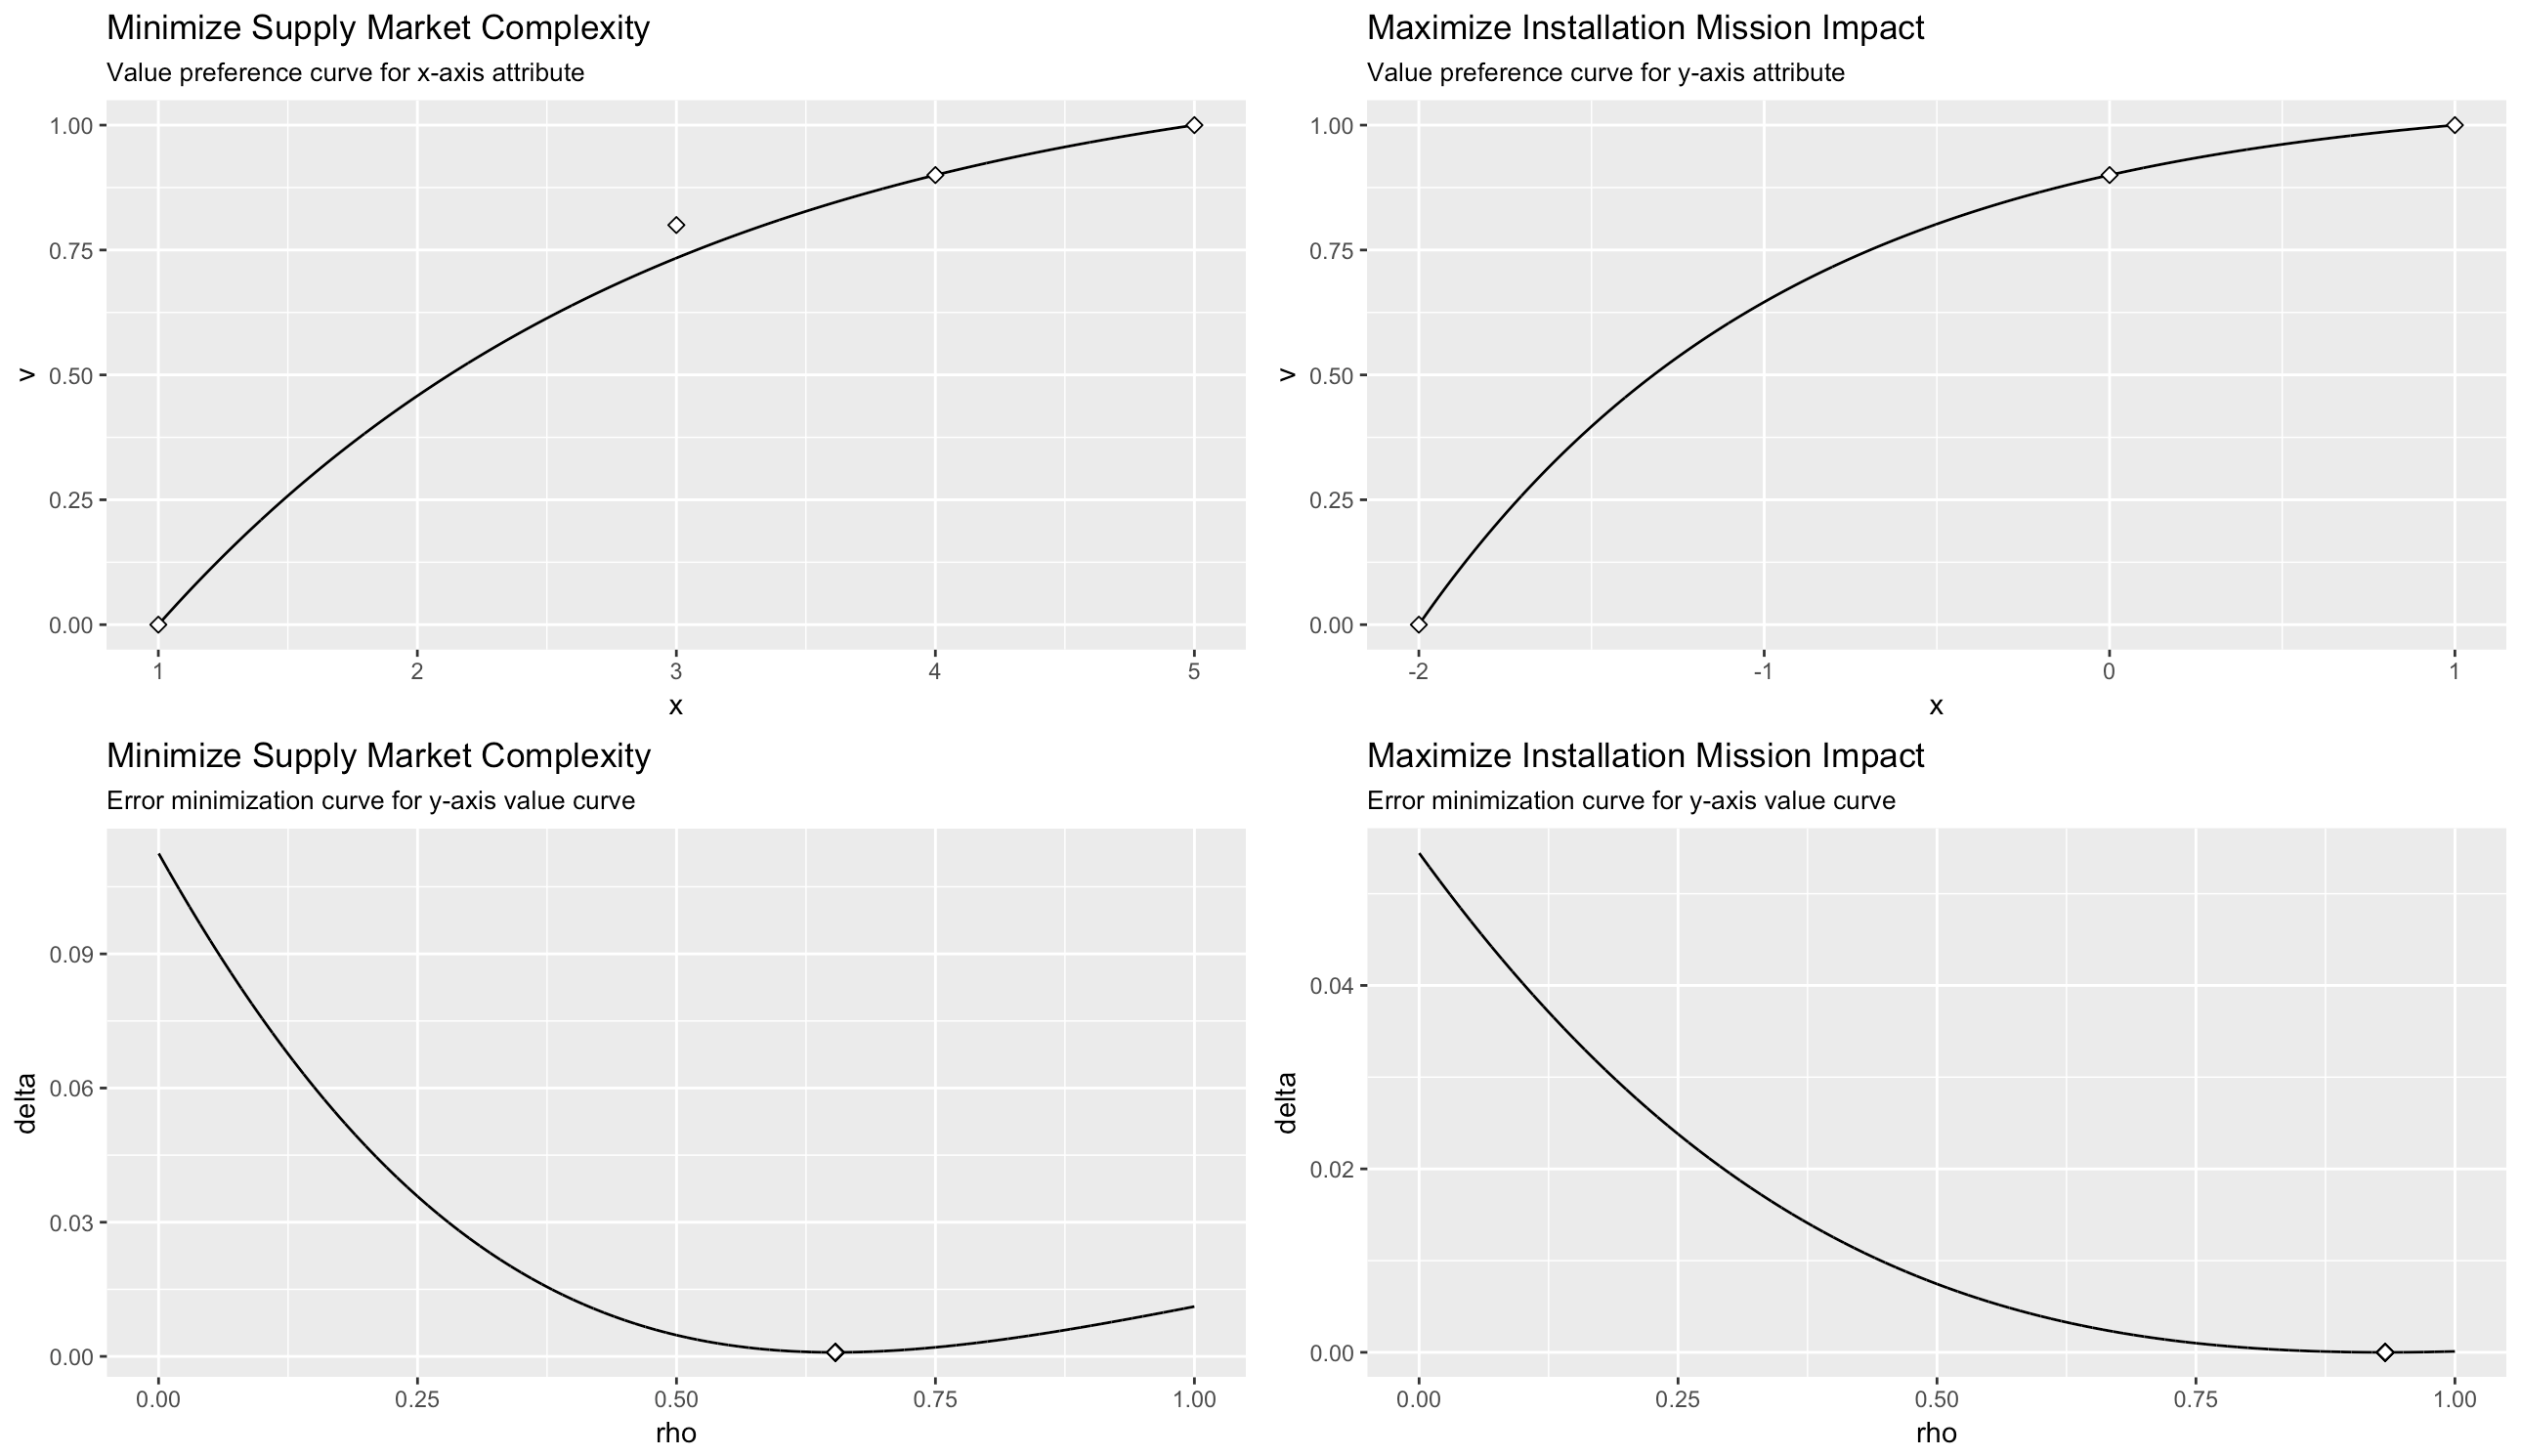
\includegraphics[width=0.5\textwidth]{fig6.png}
  \caption{Case study single attribute curves.}
  \label{fig:6}
\end{figure}

Using the identified optimal $\rho$ value for AFICA's preference curve we computed the $x$ and $y$ attribute single attribute values with the SAVF\_score function and then plotted in the KPM with the kraljic\_matrix function.

\begin{figure}[!htb]
  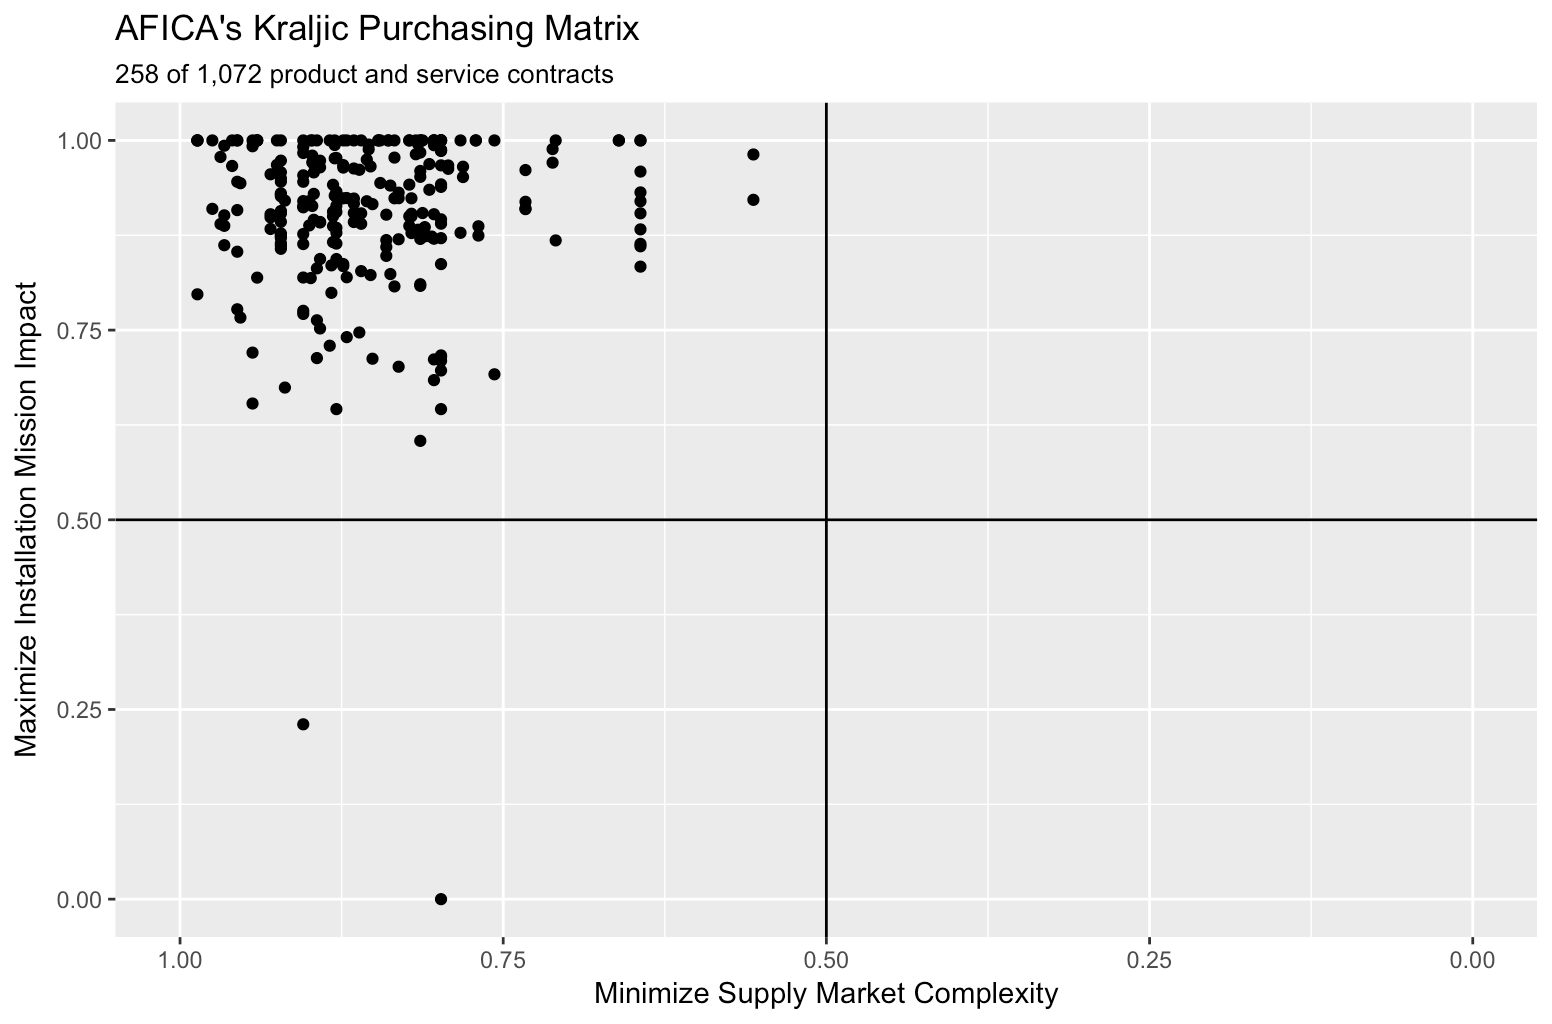
\includegraphics[width=0.5\textwidth]{fig7.png}
  \caption{Case study placement of PSCs in the Kraljic Matrix.}
  \label{fig:7}
\end{figure}

The KPM illustrates that nearly all PSCs provided by AFICA fell into the upper left (or "Leverage") quadrant.  The Leverage quadrant identifies those products and services that provide ample opportunity for cost savings by leveraging buying power.  Furthermore, it's important to note that AFICA based their selection of PSCs for this analysis on a specific set of data points they termed Key Performance Indicators, or KPIs. AFICA's KPIs were developed to identify those PSCs with the best opportunity for cost reduction. Thus we should expect to see them in the leverage quadrant. This helped to confirm that AFICA's internal analytic processes accurately identified PSCs ripe for cost reduction; this analysis provided further confirmation. Moreover, in Kraljic's seminal work of 1983, he used an example of a company that positioned 5,000 items. Only 75, or 1.5\% were positioned on the right side of the matrix (the strategic or bottleneck quadrants). Hence, such clustering of sorts is not unusual in the KPM literature. 

We note that two PSCs fall in the non-critical quadrant.  By leveraging the kraljic\_quadrant function and filtering for "Non-critical" we find that these are PSCs Z299 and 5841.  These are two PSCs that AFICA can focus on to improve efficient processes in order to reduce costs.

However, out of the remaining 256 PSCs, the question remains: Where should AFICA begin their efforts for strategic sourcing?  Here we can start to rank order the 256 PSCs that fall in the leverage quadrant with the MAVF\_score function.  Through a structured interview process with AFICA's leadership that followed the procedures discussed in Keeney, Von Winterfeldt, and Eppel (1990), we established a swing weight for the $x$ attribute to be 52\% ($w_x = 0.52$) and the swing weight for the $y$ attribute to be 48\% ($w_y = 0.48$).  Therefore, we can apply the MAVF\_score function to quickly get the top 10 PSCs for AFICA to start focusing their strategic efforts on.  

\begin{table*}[!htb]
  % table caption is above the table
  \centering
  \caption{Top 10 ranked PSCs based on MAVF score.}
  \label{tab:2}       % Give a unique label
  % For LaTeX tables use
  \begin{tabular}{ccccccc}
    \hline\noalign{\smallskip}
    PSC &	$X$ Attribute	& $Y$ Attribute	& $X$ SAVF Score & $Y$ SAVF Score	& Quadrant &	MAVF \\
    \noalign{\smallskip}\hline\noalign{\smallskip}
    7490 & 4.76 &	1.00 &	0.987 &	1.00 &	Leverage &	0.993 \\
    7520 & 4.76 &	1.00 &	0.987 &	1.00 &	Leverage &	0.993 \\
    5985 & 4.58 &	1.00 &	0.975 &	1.00 &	Leverage &	0.987 \\
    7025 &	4.37 &	1.00 &	0.959 &	1.00 &	Leverage &	0.979 \\
    5895 &	4.45 &	0.89 &	0.966 &	0.99 &	Leverage &	0.979 \\
    5820 &	4.32 &	1.00 &	0.956 &	1.00 &	Leverage &	0.977 \\
    5836 &	4.32 &	1.00 &	0.956 &	1.00 &	Leverage &	0.977 \\
    7010 &	4.49 &	0.68 &	0.969 &	0.98 &	Leverage &	0.973 \\ 
    7045 &	4.18 &	1.00 &	0.944 &	1.00 &	Leverage &	0.970 \\
    7020 &	4.14 &	1.00 &	0.940 &	1.00 &	Leverage &	0.969 \\
    \noalign{\smallskip}\hline
  \end{tabular}
\end{table*}

To check the variability of the ranking based on the swing weights we performed a sensitivity analysis via MAVF\_sensitivity allowing each swing weight to vary by $\pm 10$ (thus, $w_x = \left[0.42, 0.62\right]$ and $w_y = \left[0.38, 0.58\right]$).  The same top 10 PSCs were observed in the sensitivity analysis.  In fact the same PSCs were consistently ranked in the top 25 with only minor differences in the rank-order of PSCs in the lower half of this ranked set.  Therefore, these PSC represent those with the perceived greatest net impact to the Air Force mission and can be considered the most likely candidates for AFICA to start applying commercial best practice strategies to reduce costs.

However, it is worth mentioning that non-profit organizations such as the Air Force are often very cost sensitive.  Many times their efforts are driven not only by mission impact but also by budget constraints.  Therefore, we can gain further insights by assessing the cost-benefit trade space.   To do so, we plot each PSC relative to their five-year average cost and MAVF score as displayed in Figure 3 

\begin{figure}[!htb]
  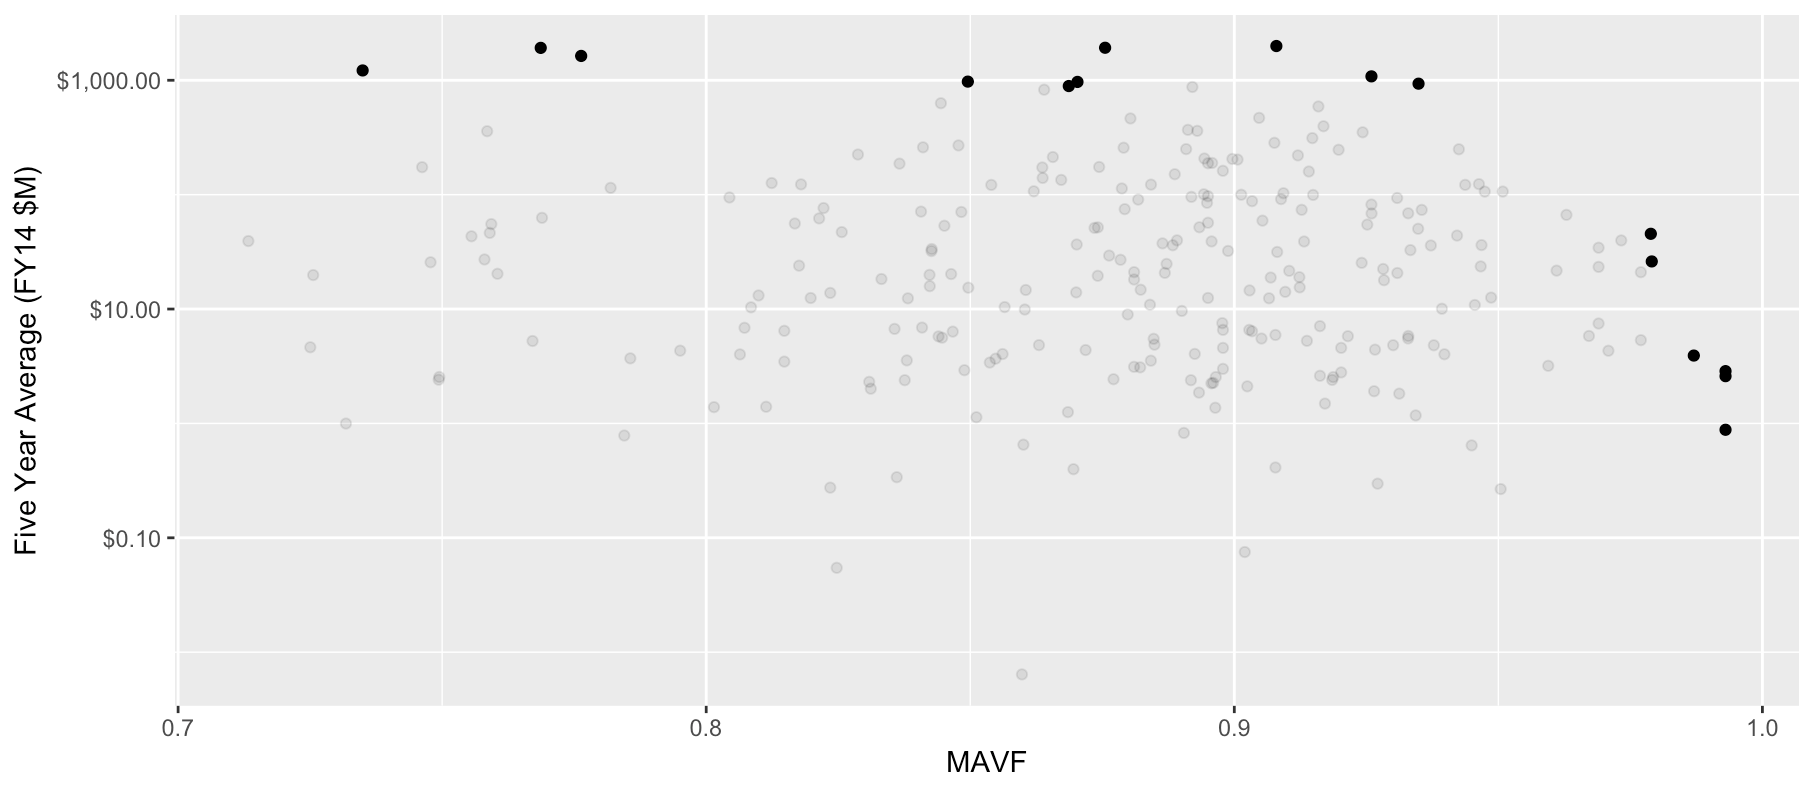
\includegraphics[width=0.5\textwidth]{fig8.png}
  \caption{Cost vs MAVF Pareto Frontier.}
  \label{fig:8}
\end{figure}

This plot, along with Table 4, illustrates the non-dominated PSCs that form the approximate Pareto frontier.   These PSCs represent those that drive maximal costs or mission impact and, therefore, represent those PSCs that are likely to be of greatest concern to Air Force leadership to further investigate for strategic sourcing opportunities.

\begin{table}[!htb]
  % table caption is above the table
  \centering
  \caption{Cost vs. MAVF Pareto Frontier PSCs.}
  \label{tab:3}       % Give a unique label
  % For LaTeX tables use
  \begin{tabular}{ccc}
    \hline\noalign{\smallskip}
    PSC &	MAVF & 5yr Avg Cost (\$M) \\
    \noalign{\smallskip}\hline\noalign{\smallskip}
    1680 &	0.73 &	\$1,219 \\
    J015 &	0.77 &	\$1,920 \\
    J016 &	0.78 &	\$1,632 \\
    2840 &	0.87 &	\$968 \\
    R414 &	0.85 &	\$973 \\
    R425 &	0.88 &	\$1,925 \\
    V126 &	0.93 &	\$934 \\
    J010 &	0.87 &	\$890 \\
    R499 &	0.91 &	\$1,992 \\
    R706 &	0.93 &	\$1,082 \\
    7025 &	0.98 &	\$26 \\
    5895 &	0.98 &	\$45 \\
    5985 &	0.99 &	\$4 \\
    7490 &	0.99 &	\$3 \\
    7520 &	0.99 &	\$3 \\
    \noalign{\smallskip}\hline
  \end{tabular}
\end{table}


%%%%%%%%%%%%%%%%%%%%%%%%%%%%%%%%%%%%%%%%%%%%%%%%%%%%%%%%%%%%%%%%%%%%%%%%%%%%%%%%
\subsection{Results}
\label{sec:5.3}
%%%%%%%%%%%%%%%%%%%%%%%%%%%%%%%%%%%%%%%%%%%%%%%%%%%%%%%%%%%%%%%%%%%%%%%%%%%%%%%%

The AFICA organization acknowledged that the data science approach to implementing this objective and quantitative approach represented a simpler and faster approach than the subjective approaches advocated in the literature and also compared to the approaches that AFICA has used in the past.  Previous iterations of subjective assessments took AFICA 30-90 days to complete.  With the KraljicMatrix package, this quantitative approach takes AFICA's analyst less than an hour to perform. When considering the data gathering and subjective measure inputs, this time increases to a week; however, this is significantly faster and more agile than previous AFICA approaches. AFICA also acknowledged that this approach led to higher quality and more insightful results than the approaches they had used in the past.  Moreover, these insights are far more reproducible when delivered in an objective and programmatic way as provided by the KraljicMatrix package.  Furthermore, without this approach being deployed in an open source capability such as R, AFICA acknowledged that their limited analytic resources would likely have constrained them from actually being able to implement the solution.  The AFICA leadership team is excited about the time and effort savings that this new approach represents and views this new analytic capability as an essential way of providing a reliable, objective, and consistent approach to quantitatively analyze strategic sourcing.


%%%%%%%%%%%%%%%%%%%%%%%%%%%%%%%%%%%%%%%%%%%%%%%%%%%%%%%%%%%%%%%%%%%%%%%%%%%%%%%%
\section{Conclusions}
%%%%%%%%%%%%%%%%%%%%%%%%%%%%%%%%%%%%%%%%%%%%%%%%%%%%%%%%%%%%%%%%%%%%%%%%%%%%%%%%

This research provides two important contributions. First, extant research has largely focused on advancements in large and complex data, emerging analytic techniques, and how organizations and education are changing in the age of big data analytics.  However, a significant gap exists in the practicality of OR research \citep{hsbh16} and illustrations of exemplar case studies to illustrate how academics and organizations can deploy analytic applications \citep{gh14,p14,wgnp16}.  Furthermore, despite the call for research to demonstrate data science capabilities across the supply chain \citep{wf13}, minimal research exhibiting this aptitude has been produced.  This research contributes by demonstrating how data science and open source technology can be used to develop, automate, and deploy analytic techniques to help meet the growing demand of data-driven decision making across organizational processes.

Second, past research has identified a lack of quantitative approaches to position items in the Kraljic Matrix \citep{pwa12,wj04,ktp14}.  Furthermore, for the few quantitative approaches that have been proposed, the ability to extend and deploy them for practical use has been difficult and limited \citep{dpbhc08,pbtj13}. This research demonstrates a simple and practical multi-objective approach for positioning and analyzing a firm's purchasing portfolio. Furthermore, by deploying this quantitative framework in an R package environment, distribution and implementation of the approach is efficient, effective, and practical.

Combined, this research illustrates how data science can be used to not only advance analytic approaches to problems but also to deploy them across academic and industry organizations for practical application.

On behalf of all authors, the corresponding author states that there is no conflict of interest.


%%%%%%%%%%%%%%%%%%%%%%%%%%%%%%%%%%%%%%%%%%%%%%%%%%%%%%%%%%%%%%%%%%%%%%%%%%%%%%%%

\begin{acknowledgements}
TBD.
\end{acknowledgements}

% BibTeX users please use one of
\bibliographystyle{spbasic}      % basic style, author-year citations
%\bibliographystyle{spmpsci}      % mathematics and physical sciences
%\bibliographystyle{spphys}       % APS-like style for physics
\bibliography{boehmke-ijdsa-2017}   % name your BibTeX data base

\end{document}
% end of file template.tex

